
%\documentclass[onecolumn,prl,nobalancelastpage,aps,10pt]{revtex4-1}

%\documentclass[rmp,preprint]{revtex4-1}

\documentclass[11pt]{article} % Try also "scrartcl" or "paper"
\linespread{1.5}
 \usepackage[margin=3cm]{geometry}   % to change margins
 \usepackage{titling,cite,subfig}             % Uncomment both to   
 \setlength{\droptitle}{0cm}     % change title position 
\title{%\vspace{-1.5cm}            % Another way to do
Feature Descriptors for Gait Analysis From Depth Sensors}
\usepackage{graphicx,bm,subfig,amsmath,amsfonts,listings,url}
\usepackage{gensymb}
\usepackage{color}
\usepackage{titlesec}
\usepackage{hyperref}
\usepackage[toc,page]{appendix}
 \usepackage{booktabs}
 \usepackage[table,xcdraw]{xcolor}
\titleclass{\subsubsubsection}{straight}[\subsection]
\usepackage{epstopdf}
\usepackage{longtable}
\newcounter{subsubsubsection}[subsubsection]
\renewcommand\thesubsubsubsection{\thesubsubsection.\arabic{subsubsubsection}}
\renewcommand\theparagraph{\thesubsubsubsection.\arabic{paragraph}} % optional; useful if paragraphs are to be numbered

\titleformat{\subsubsubsection}
  {\normalfont\normalsize\bfseries}{\thesubsubsubsection}{1em}{}
\titlespacing*{\subsubsubsection}
{0pt}{3.25ex plus 1ex minus .2ex}{1.5ex plus .2ex}

\makeatletter
\renewcommand\paragraph{\@startsection{paragraph}{5}{\z@}%
  {3.25ex \@plus1ex \@minus.2ex}%
  {-1em}%
  {\normalfont\normalsize\bfseries}}
\renewcommand\subparagraph{\@startsection{subparagraph}{6}{\parindent}%
  {3.25ex \@plus1ex \@minus .2ex}%
  {-1em}%
  {\normalfont\normalsize\bfseries}}
\def\toclevel@subsubsubsection{4}
\def\toclevel@paragraph{5}
\def\toclevel@paragraph{6}
\def\l@subsubsubsection{\@dottedtocline{4}{7em}{4em}}
\def\l@paragraph{\@dottedtocline{5}{10em}{5em}}
\def\l@subparagraph{\@dottedtocline{6}{14em}{6em}}
\makeatother

\setcounter{secnumdepth}{4}
\setcounter{tocdepth}{4}


\usepackage{microtype}

%\renewcommand{\thesection}{\arabic{section}}
%\renewcommand{\thesubsection}{\thesection.\arabic{subsection}}
%\renewcommand{\thesubsubsection}{\thesubsection.\arabic{subsubsection}}
\DeclareMathOperator*{\argmin}{arg\,min}
% Fix references
\makeatletter
\renewcommand{\p@subsection}{}
\renewcommand{\p@subsubsection}{}
\makeatother

\usepackage{bibentry}
\usepackage{pdfpages}

\newcommand{\comment}[1]{}
\begin{document}
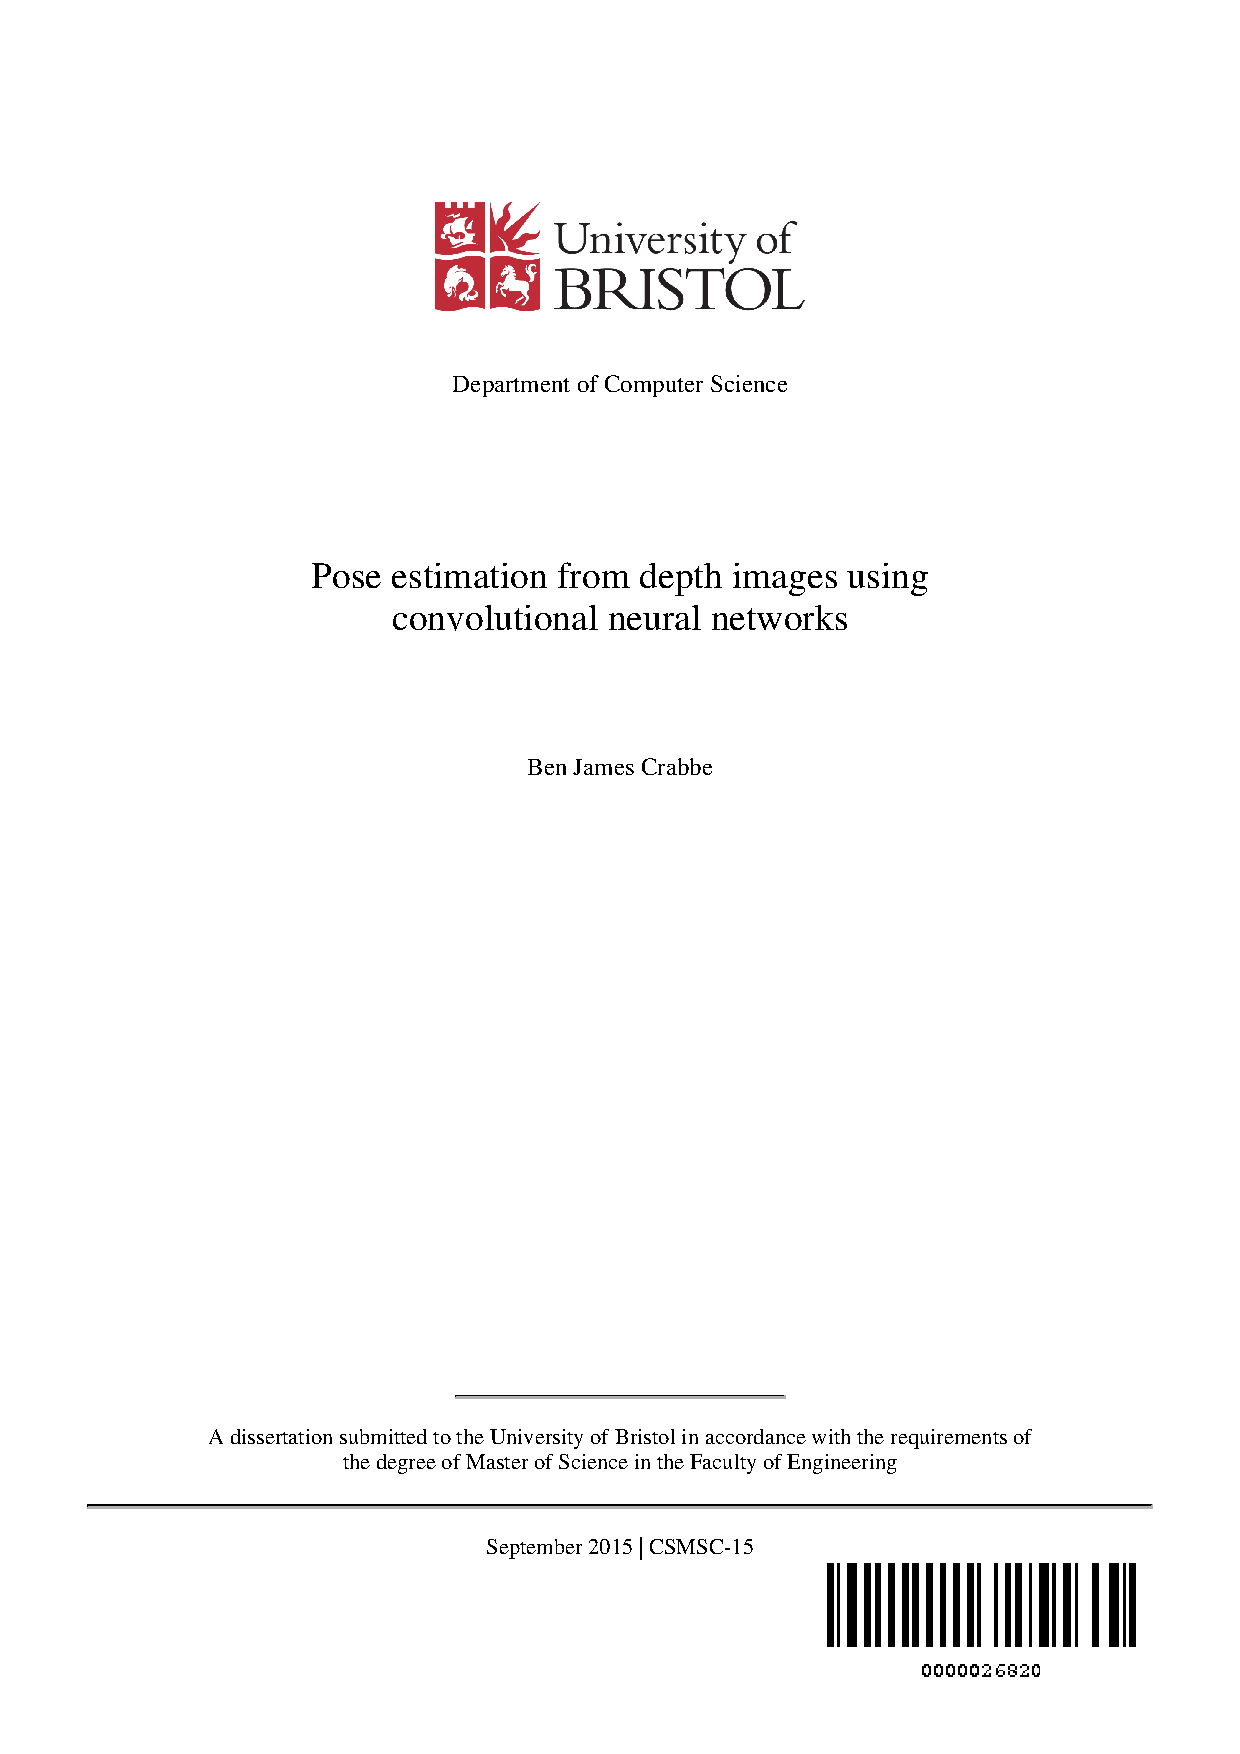
\includepdf[pages={1,2}]{frontcover}

%/maketitle
\tableofcontents
\comment{

A statement of the aims and objectives of the project.


A description of the background and context of the project and its relation to work already done in the area. (Note that while you are free to re-use work from your research review here, it would normally be appropriate to tailor your earlier work to better suport the final contributions of the project. Typically you will include new related work which was found to be important, while excluding previously studied work which has become irrelevant, and modifying your earlier write-up with more or less detail, as required).



A description of the work carried out. This should include details of technical or scientific problems tackled, solutions proposed, and the design and development of software.



A description and analysis of results obtained.



A critical evaluation of the work. This is an analysis of the extent to which the project has achieved its objectives, and whether the choices that were made were, with hindsight, the best ones.
Suggestions on possible improvements and/or further work.


	Introduction:
		Discuss SPHERE, the need for in home gait analysis, references that show this is possible from kinect, 
	The existing pipeline:
		Kinect SDK skeletons... shotton et al.
		same as lit review, but go into more detail on the dimensionality reduction/manifold method
	

}







\section{Introduction}

%SPHERE - a Sensor Platform for Healthcare in a Residential Environment, is a interdisciplinary research project being undertaken in Bristol which aims to help solve some of the problems currently faced by the healthcare system in the UK. The goal is to design a range of sensors to be fitted in residential environments that facilitate the care and rehabilitation of inhabitants. 
 %reference for some medical textbook?
%A Kinect Based Approach to Assist in the Diagnosis and Quantification of Parkinson’s Disease
%R. Torres, M. Huerta, R. Clotet, R. González, L. E. Sánchez, D. Rivas, M. Erazo
%Parkinson’s Disease (PD) is a degenerative process of the central nervous system. Its main body symptoms are tremors, rigidity, bradykinesia and walking difficulty. These symptoms may increase and so it is necessary to have a constant and successful evaluation, so the PD patient may receive the appropriate treatment. There are systems that enable the monitoring of tremors based on sensors, most of them attached to the patient’s body. Some such systems comprise accelerometers or use of Nintendo Wii Remote sensors (NWR). As a proposal that allows true portability, without the attachment of a single sensor to the patient’s body, or need for batteries, this paper introduces a pilot system that allows to diagnose PD and evaluate its severity using Kinect sensors.

Gait analysis plays an important part in the treatment and assessment of a number of medical conditions. At present gait analysis is usually performed through a combination of visual assessment by an experienced physiotherapist, automated methods such as marker based motion capture, pressure sensitive walkways or accelerometers. It generally involves travelling to a gait assessment laboratory and this can be an issue for patients who have difficulty walking. 

This problem, and a range of other healthcare challenges, are being tackled through research and development by the SPHERE (a Sensor Platform for Healthcare in a Residential Environment) group in Bristol. An automatic, in home, gait analysis pipeline has been designed~\cite{Paiement,Tao} which assesses the quality of a subjects movement using data captured by the human pose estimation (skeleton/joint tracking) systems implemented by RGB-D cameras such as the Microsoft Kinect.

The system uses data driven, machine learning methods to learn both a low dimensional representation of pose\footnote{The points in this space are referred to as the pose vector, and the Kinect skeleton data as the body configuration or joint position vector.} and models of normal motion from which it quantifies the quality of movement. Because of this, it can be applied naturally to other types of movement quality assessment such as sports movement optimisation or physiotherapy exercise coaching. The system has been applied to a sitting-standing motion, to punching motions in boxing~\cite{SPHEREweb} and to people walking up stairs~\cite{Paiement,Tao}.

One issue currently limiting the effectiveness of this system is the fragility of the skeleton tracking software. This software was designed for controlling entertainment/gaming systems with the user viewed frontally, within a range of 1-4m and at a pitch angle near 0$\degree$. Outside of these conditions skeletons become noisy and unreliable. Typically only a small fraction of data recorded from a camera fixed $\sim$1.5m above the top of stairs is fit for use with the system. Increasing the fraction of usable data requires more intrusive camera placement which is to be avoided. The skeleton tracker also performs poorly when props are involved, for example grasping a banister or a ball often leads to erroneous joint positions for that arm. It also struggles to accurately record sitting/standing motions which is a key motion hoping to be analysed in SPHERE homes.

The aim of this project was to develop a system for determining the low dimensional pose representation used in~\cite{Paiement} directly from RGB-D footage, with the additional aims that the system should be naturally applicable to a range of motions and able to maintain reasonable accuracy at a range of viewing angles. The methodology we found most suited to this task was a convolutional neural network (CNN). CNN's are a supervised learning method for extracting features, e.g. the pose vector, from images. After training the network is able to generalise to unseen data, producing an output inferred from the examples it has seen. This method effectively learns the feature representations that produce the most accurate regression. The advantage of this over traditional hand crafted feature extraction is that when applied to new motions the type of features extracted will be re-tuned to better capture the pose vector from the data of the new motion.

One restriction of CNN's is that they require a large amount of data to be trained effectively. In this project, as in~\cite{Paiement,Tao} we have focused on an analysis of the stair ascent motion as this was the only existing dataset of the required size. We use the joint position data captured by the Kinect to produce the ground truth pose vectors used to train the CNN. The Kinect skeletons are not ideal ground truth; by using them we are restricted to only motions which the Kinect is able to capture. Also, their errors and imprecision produce an inconsistent mapping between similar images and labelled pose vectors which can confuse the network. Despite this we find that in a majority of cases the CNN is able to match the Kinect measurement to a high degree, and in some cases predict poses which correspond better to what is seen in the images than was produced by the Kinect. The accuracy of the CNN is measured by the distance (euclidean/L2 norm) between its predicted point and the ground truth. This is used during training as a objective/loss function and in the analysis of the final performance. The effect of using the CNN's pose measurements for the movement quality analysis of~\cite{Paiement,Tao} is also examined. Comparing it to that of the ground truth we find that in some cases the network predictions are actually more adept at producing the correct abnormality than the Kinect skeletons.

In Section \ref{sec:bg} we present an introduction to depth imaging, human pose estimation and convolutional neural networks. In Section \ref{sec:methods} we detail the steps used to achieve our results. In Section \ref{sec:results} we present and analyse our results. In Section \ref{sec:discussion} we evaluate the suitability of our chosen method and present suggested directions for future work.






\section{Background and Related Work}
\label{sec:bg}
\subsection{Depth Imaging}
\label{sec:Depth}


In depth images each pixel value represents the distance of that point from the camera. Depth images are unaffected by changes in lighting or human appearance. They provide a 3D map of the scene, making background-foreground separation far easier. These features can often simplify computer vision tasks, particularly human pose estimation~\cite{Chen2013}.

There are three main technologies used to produce depth images: Time~of~flight~(ToF) cameras, Stereo~imaging cameras and Structured~light cameras. It was not until the last~5~years that affordable good~quality and easy to use depth sensors came on the market and since then there has been an explosion in their use in the computer vision community~\cite{Han2013}.

The data in the SPHERE staircase dataset was captured using a Asus Xtion Pro Live which uses the structured light technology developed by Primesense (same as the Microsoft Kinect). It consists of an infrared laser emitter and an infrared camera, which together make up the depth sensor, and a RGB camera. An infrared laser is passed through a diffraction grating to produce a known pattern of dots that is projected onto the scene then reflected back and captured by the infrared camera. The measured pattern is compared to a reference pattern produced at a known distance of reflection, which has been stored during the calibration process. The surface of reflection being farther or nearer than the reference surface produces a shift in the pattern which is used to determine the depth value~\cite{Zhang2012a,Khoshelham2012a} as shown in figure \ref{fig:kinectMeasure}.

\begin{figure}
\centering
\includegraphics*[width=0.45\linewidth,clip,trim={1.2cm 1cm 0.7cm 1.5cm}]{kinectMeasure}%
\caption{The process by which depth is computed from triangulation of structured light. From \cite{Han2013}		\label{fig:kinectMeasure}}
\end{figure}

\subsubsection{Sensor Performance}
\label{sec:senPerf}

Most of the studies reported below have focused on the Microsoft Kinect however the Asus Xtion Pro uses the same depth sensing system. When the two were compared in~\cite{Gonzalez-Jorge2013} they were shown to perform equivalently, hence we report the findings based on Kinect performance.

The range of the depth sensor is~0.8-3.5m with increasingly noisy or incomplete readings up to 8m. It has a~43$\degree$~vertical by~57$\degree$~horizontal field~of~view~\cite{Han2013} and captures 640 $\times$ 480 depth images.

Stoyanov et al.~\cite{StoyanovTodorandLouloudiAthanasiaandAndreassonHenrikandLilienthal2011a} compare the performance of the Kinect with that of two other ToF depth imaging cameras (SwissRanger~SR-4000 and Fotonic~B70~ToF) assessing them against a ground truth of expensive and low fps laser depth scanner measurements. They find that within a range of 3.5m the Kinect outperforms the ToF sensors and is comparable to the laser scanner, outside of this range the accuracy falls considerably.

Both Khoshelham~\&~Elberink~\cite{Khoshelham2012a} and Smisek~et~al.~\cite{Smisek2011} have measured this effect experimentally comparing Kinect measurements with those from high performance laser scanners. They find that temporally fluctuating noise in the depth measurements increases quadratically with distance from the sensor so the depth precision decreases from around~±0.5cm~at~1m to~±7cm at~7m. Nguyen~et~al. shows that noise increases linearly with lateral distance, and is greatly increased on surfaces at greater than 70$\degree$~angles~\cite{Nguyen2012}. This last effect can lead to increased levels of noise around edges of humans. 

As well as noise the structured light sensors often return 'unknown' depth value pixels, known as holes, when the infrared receiver cannot read the reflected pattern properly. This can occur around the sides of foreground objects due to the slightly different viewing angles between the projector and camera as in regions 2~and~3 of figure~\ref{fig:kinectHoles4}, or when certain surface materials, such as human hair, interfere with the infrared pattern's reflection as in region~4 in figure~\ref{fig:kinectHoles3}. 
 \begin{figure}
\includegraphics*[width=1\linewidth,clip,trim={1cm 1.5cm 1cm 1cm}]{kinectHoles4}
\caption{Shows the holes in structured light depth data due to the different perspectives of IR projector and senor (regions~1~and~3) and due to the surface of reflection being roughly~5m away and at a large angle(region~2) From~\cite{Feng2013}		\label{fig:kinectHoles4}  } 
\end{figure}
 \begin{figure}
\includegraphics*[width=1\linewidth,clip,trim={1cm 1.5cm 1cm 1cm}]{kinectHoles3}
\caption{Shows the holes in depth data due abnormal reflections from certain glossy surfaces like the TV monitor and the subjects hair.  From~\cite{Feng2013}			\label{fig:kinectHoles3}  } 
\end{figure}

%It should be noted that each of these studies mentioned above~\cite{Khoshelham2012a,Smisek2011,Nguyen2012} fail to consider the environmental factors in the quality of the measurement. Fiedler~\&~Muller \cite{Fiedler2013} show that air draft can cause changes of the depth values up to~21mm at a distance of~1.5m, and temperature variations cause changes up to~1.88mm~per~1$\degree$~C. They also find a temperature dependant drift in the position of objects captured by the RGB camera.

\subsection{Human Pose Estimation}

Human pose estimation (HPE) is generally considered as the task of measuring in 2D or 3D the joint positions of the human body. It is one of the most researched problems in computer vision because of its difficulty and due to its use in a variety of applications such as video surveillance, human–computer interaction, digital entertainment, sport science and medical applications.

This is a difficult task for a number of reasons. Firstly the human body has around 20 degrees of freedom~\cite{Forsyth2005}, producing a huge space of possible body configurations, many of which will cause some joints to be occluded when viewed from a single camera. Additional difficulties arise from the variety in human appearance and clothing, and from left right ambiguities. Traditional motion capture methods (MoCap) rely on markers attached to the subject and multiple cameras to overcome these issues. Whilst such systems can provide highly accurate pose data, their use is restricted to controlled environments using expensive and calibrated recording equipment which renders them unsuitable in many applications.

Monocular visual pose estimation methods (reviewed in \cite{Moeslund2006, Hen2009,Poppe2007,Sminchisescu2006,Liu2015}) are generally divided into two approaches (e.g. by \cite{Poppe2007}); model based (or generative) and model-free (or discriminative) approaches. Model based approaches use prior knowledge of human shape and kinematics such as fixed limb lengths and defined joint angle limits to cast the image to pose transformation as a nonlinear optimisation problem or probabilistically in terms of a likelihood function, i.e. given this image data (and sometimes previous frames pose knowledge) what is the most likely valid pose. Model-free approaches instead learn a direct mapping from image data to pose, generally requiring learning/example based methods to achieve this. Some 'hybrid' approaches combine the two using model-free methods as an initialiser to model based methods. 


\subsubsection{Human Pose Estimation Using Dimensionality Reduction}

With both of the above approaches there are significant issues posed by the high dimensionality of pose data. In model based approaches likelihood functions, which are usually multi-modal and non-Gaussian, require a randomised search~\cite{Sminchisescu2003}. Such searches in~20 dimensions are computationally expensive and often lead to super real time frame rates~\cite{Hen2009}. In model free approaches training data must account for the highly non-linear mapping between image and pose, which means that the pose space must be densely sampled in the training set. Densely sampling a 20 dimensional space, even just the parts that correspond to valid human motion, whilst also modelling all the invariant aspects such as body shapes, viewing angle etc requires an inordinate amount of data~\cite{Hen2009,Agarwal2006}.%Agarwal2006Recovering 3D human pose from monocular images

Although the full pose space is very large and high dimensional it has been shown e.g. in \cite{Brand1999,Elgammal2004} that when considering only movements in a well defined activity such as walking, then the pose data can be well represented by a low dimensional latent manifold; this strategy was used in the SPHERE work~\cite{Paiement}. In a work closely related to our own Elgammal et al. \cite{Elgammal2004} use Local Linear Embedding (LLE), a dimensionality reduction method, to generate a 1D manifold representation (embedded within a 3D space), shown in figure~\ref{fig:elg}, of a walking motion from single sequences of silhouette images. They use a Generalised Radial Basis Function interpolation framework~\cite{Poggio1990} (a form of neural network) to learn two mappings, one from the manifold to the silhouette image space and another from the manifold to full 3D joint positions. They then invert these mappings to extract points on the manifold from silhouettes and 3D joint positions from the points on the manifold. In contrast, our work builds the manifold representation from 3D joint position data, this has the benefit of the manifold representation not being tied to subject's visual appearance. This allows it to generalise naturally to multiple subjects, which is not the case in~\cite{Elgammal2004} (although they do introduce an solution for this problem in~\cite{Elgammal2004a}). It is also unlikely that this method could be used to capture abnormality in gait since defining an image to manifold transformation explicitly from the inverse constrains all input images to the poses contained in the original data. Elgammal et al. argue that learning a smooth mapping from examples is an ill-posed problem unless the mapping is constrained since the mapping will be undefined in other parts of the space. We address this issue in section~\ref{sec:abnormals}.
\begin{figure}
\centering
\includegraphics*[width=0.6\linewidth,clip]{elgamel}
\caption{ The 1D gait manifold produced from LLE dimensionality reduction on images of shilouttes used by Elgammal et al. to simplify joint tracking. From~\cite{Elgammal2004}. \label{fig:elg}  } 
\end{figure}



Brand \cite{Brand1999}, also inferred 3D pose from silhouettes using an intermediate manifold representation. He uses a maximum a posteriori estimation for mapping between the image and manifold space. This uses information across the whole input sequence to find the most likely and consistent solutions in order resolve the ambiguities in the many to many silhouette to pose mapping. A solution of this form is unacceptable in our case as one of the key features of the SPHERE system is online measurement.

Similarly Urtasan et al. \cite{Urtasun2005} used Scaled Gaussian Process Latent Variable Models (SGPLVM) \cite{Lawrence2004} on single training sequences (walking and a golf swing) labelled with 2D joint positions. These models build a low dimensional manifold, and simultaneously, a continuous mapping between this and the 2D joint positions. They use the low dimensional representation to facilitate efficient maximum a posteriori based tracking in this space. Again, this is only suitable as an offline solution. 

Tangkuampien and Suter \cite{Tangkuampien2006} used Kernel Principle Component Analysis (KPCA) to learn low dimensional representations of 3D joint positions, and separately using the same method, a low dimensional representation of silhouette images. They then learn a mapping between these spaces using Locally Linear Embedding (LLE) reconstruction.% This has some similarity with our own approach of using a CNN, where the image is transformed in to progressively more concise feature representations, before the regression takes place. The disadvantage of using LLE to perform the final transformation is that it is restricted to within the manifold space contained in pose training data. %As discussed above, our method has the benefit that it naturally maps unseen poses away from the manifold of the training data. This reduces the number of poses we must capture in our training data.

Rosales et al \cite{Rosales2000,Rosales2001} used 3D joint position data from a MoCap system to render synthetic training data from multiple angles. Hu moments were used to extract visual features from these (and real) images. Unsupervised learning was used to cluster 3D joint position data into areas of similar pose and a neural network was trained separately on each cluster to learn the mapping from visual features to pose. Using the developments in training of deep neural networks since this work we show that it is feasible to have a single CNN learn both the features best suited and the mapping to all poses. This removes the need for clustering and separate networks leading to a simpler, easily adaptable solution. Their use of MoCap data as opposed to Kinect Skeletons for ground truth is a change we could expect to improve performance in our system. Similarly rendering synthetic training data from multiple angles would be a smart way of improving our viewing angle tolerance.

\subsubsection{Human Pose Estimation From Depth Images}

Challenging aspects of RGB HPE such as the variability in human appearance and scene lighting were greatly simplified with the advent of low cost commodity depth sensors. RGB-D also provides richer data for inferring 3D structure, allowing human poses which could appear identical when projected onto a 2D image plane to be distinguished. Full body HPE methods from single depth images are reviewed in \cite{Helten2013}. With the Kinect/Xtion sensor and software packages (Kinect SDK or alternatively the open source OpenNI) low cost, flexible and reasonably accurate HPE is now available and has been employed in a huge variety of scientific applications~\cite{Han2013,Giovanni}.

The Kinect SDK and OpenNI skeleton trackers apply some inter-frame tracking algorithms to the single frame pose measurements of~\cite{Blake2011}. In this work Shotton et al. leveraged a large MoCap 3D joint position dataset which they re-targeted onto a variety of synthetic body models before rendering as if captured from a Kinect, simulating sensor noise, camera pose, and crop position. Producing synthetic depth images data is far simpler than in RGB since depth is far more invariant to subject clothing and appearance changes. Using these generated depth images and a ground truth labelling of each pixel as one of 31 body parts they trained a randomised regression forest to perform this body part classification at each pixel using simple and computationally efficient pixel wise depth comparison features 
\begin{equation}
f(\boldsymbol{u} \mid \boldsymbol{\phi}) = z(\boldsymbol{u}+\frac{\boldsymbol{\delta}_1}{z(\boldsymbol{u})})-z(\boldsymbol{u}+\frac{\boldsymbol{\delta}_2}{z(\boldsymbol{u})})
\label{eq:dcf}
\end{equation}
where $\boldsymbol{u}$ is a pixel location, $\boldsymbol{\phi}$ is two randomly generated 2D offsets $\boldsymbol{\delta}_1$, $\boldsymbol{\delta}_2$ , $z(x,y)$ is a function which returns the depth at the input location. Examples of these features are shown in figure \ref{fig:dcf}.

\begin{figure}
\centering
\includegraphics*[width=0.6\linewidth,clip]{kinectFeature}
\caption{An example the depth comparison features from equation \ref{eq:dcf} used in \cite{Blake2011} to perform per pixel body part classification. The yellow crosses indicate the image pixel $\boldsymbol{u}$ being classified. The red circles indicate the offset pixels as defined in equation \ref{eq:dcf}. They use random forests which combine many such features to give a strong discriminative signal. From~\cite{Blake2011} \label{fig:dcf}  } 
\end{figure}

They then use these classifications to infer actual joint position through a simple averaging and mean shift procedure. The whole algorithm operates in real time on the computational resources allowed to them on the Xbox gaming consoles GPU. \cite{Shotton2013a} adapts this work by allowing pixel classifications of a number of surrounding joints to be used when estimating the joint position, rather than the single corresponding body part pixels as in~\cite{Blake2011}. This is shown to improve the quality of the prediction for occluded joints. A similar use of MoCap joint position data for rendering synthetic images from multiple views we suggest as an ideal way for increasing the view angle and subject invariance of our system.

%Another discriminative method is \cite{Plagemann2010} where they find geodesic extrema (which are expected to correspond to the feet, hands and head) on a graph produced by connecting all depth pixels in the image into a map. These points are identified (as hands feet or head) by applying local shape descriptors around the area. 

Other methods e.g.~\cite{Ye2011,Wei2011,Baak2011,Zhu2008} have focused on improving temporal smoothness of the measured pose by combining such discriminative methods with model based temporal tracking methods. 

In a recent attempt Chan et al \cite{Chan2014} use 3D point cloud information and propose a viewpoint and shape histogram feature based off these point clouds. This feature is then used to categorise the pose based on the action being performed using an introduced action mixed model. Each action is prescribed its own low dimensional manifold which allows a human pose database containing a limited amount of data to probabilistically infer the full pose.
%look at He2015




\subsection{Convolutional Neural Networks}

Convolutional Neural Networks (CNNs) are biologically inspired supervised learning systems for extracting features from locally correlated inputs such as images or sound. Essentially their goal is to learn an approximation of the function
\begin{equation}
\boldsymbol{Y} = F(\boldsymbol{Z},\boldsymbol{W})
\label{eq:networkF}
\end{equation}
where~$\boldsymbol{Z}$ is an input vector, the output~$\boldsymbol{Y}$ is the extracted feature, in our case the inferred pose vector of an image, and~$\boldsymbol{W}$ are the trainable parameters of the network. 
 
They consist of a set of filter maps, essentially matrices (or tensors if applying to multiple channels), which are applied repeatedly (convolved) across the whole of the input. Each application of these filters produces an activation value which is the sum of each filter element multiplied by its corresponding input pixel value plus a shift term known as a bias. The filter is applied iteratively across the whole image, typically with some overlap. This builds up an `activation map' for that filter, with each layer being comprised of a number of filters. The activations of each filter are stacked together, becoming the new image which is passed onto the next layer. This process is illustrated in figure \ref{fig:convnet}. This type of layer, known as Convolution layers, are typically followed by a non-linear function which is what enables the CNN to learn non-linear transformations such as the image to pose transformation we require. Although it is possible to stack convolutional layers on top of each other they are often followed by a pooling layer (also called subsampling). The idea of pooling is to reduce the spatial size from the previous layer as seen in figure~\ref{fig:pool}. Operating on each depth slice individually, i.e. each filter's activation map, the pooling window moves across the image taking the values of the elements in the input, conglomerating them using some operation, typically taking the max value as seen in the right hand side of figure~\ref{fig:pool}. CNNs also typically contain one or more fully connected layers at the end. Being fully connected means that rather than having a small filter applied repeatedly across the input, a number of filters of the same dimensions as the input are applied to the whole volume. This then outputs a~$1\times 1 \times K$ volume where~$K$ is the number of filters. This is then identical to regular neural networks where each unit in a layer is connected to every unit in the next. In our case, fully connected layers take the final high level feature representation from the rest of the network and perform the final regression to the pose vector. 

\begin{figure}
\includegraphics*[width=1\linewidth,clip]{convnet}
\caption{Shows a representation of the activations produced following a number of convolution layers, non-linearities (Rectified Linear Units, or ReLUs, are the function $max(0,x)$) and pooling layers. The network, an online demo from \cite{KarLects}, is classifying images from the CIFAR-10 dataset using the ConvnetJS library\protect\footnotemark.  \label{fig:convnet}  }
\end{figure}
\footnotetext{http://cs.stanford.edu/people/karpathy/convnetjs/}

\begin{figure}
\includegraphics*[width=1\linewidth,clip]{pooling}
\caption{Shows the effect of pooling layers in a CNN.  From~\cite{KarLects} \label{fig:pool}  } 
\end{figure}

CNNs are trained using backpropagation and gradient descent. During training an error function is defined which quantifies the difference between the networks output and the desired output. In our case, as is typical of regression tasks, we use the squared euclidean distance between the two. Using the backpropagation algorithm~\cite{Rumelhart1986} the derivative of this error with respect to each parameter is found.  Then the values of each parameter are adjusted a small amount in the direction which reduces the error. In this way, over many training examples, the network converges on a minima in the error surface across the space of all parameter values.  A derivation of the backpropagation equations and extensive technical discussion of CNNs can be found in the preceding work on this project~\cite{Crabbe2015}.

An advantage of CNNs over traditional computer vision methods is that rather than prescribing a hand-engineered feature such as the depth disparity feature in~\cite{Blake2011} or the view point and shape feature of~\cite{Chan2014}, the network is responsible for learning features itself based off the data. This presents a significant advantage in our application since features which might be good for measuring pose for one type of motion may not be useful for other motions. %

Deep CNNs have a proven capacity to learn a huge number of different visual representations. They have achieved great success in the International Large Scale Visual Recognition Challenge (ILSVRC, or ImageNet challenge) which is conducted each year and requires identification and localisation (separately) of 1000 different types of object. The work of~\cite{Krizhevsky2012} showed how deep networks could be trained by using ReLU non-linearities in place of the previous staple of tanh or logisitic functions, this over came the vanishing gradient problem that had previously made large network infeasible. Since then CNNs have achieved the best results in each task every year running, with every single participating team using them by 2014~\cite{Russakovsky}.

Training deep networks requires a large amount of data. Without this the network may begin to over fit the training data. When this occurs the errors for the network on inputs not in the training set, known as the test set, increases. It can be shown~\cite{Seung1992,Vapnik1994} that the difference between the errors on test set and those on the training set is related to both the size of the training set,~$P$, and the capacity,~$c$,  of the network i.e. 
\begin{equation}
E_{test}-E_{training} \propto \frac{c}{P}
\label{eq:errorCap}
\end{equation}
The capacity of the network is essentially the number of parameters being trained, which depends on the number of layers, the dimensions of the input images and the number of channels, the size and number of convolving filters and the way the filters and the pooling are applied. Increasing capacity will also decrease the size of~$\boldsymbol{E}_{training}$, hence there the aim in designing the network is to find the architecture which minimises both~$\boldsymbol{E}_{training}$ and~$\boldsymbol{E}_{test}-\boldsymbol{E}_{training}$ as far as possible~\cite{LeCun1998}.

Since ImageNet contains around 15 million training examples it has enabled the training of very large networks such as the 2014 winner GoogLeNet which had 22 layers~\cite{Szegedy2014}. In our case we are limited by the size of our dataset which contains a total of 6228 usable examples, many of which are practically identical due to being adjacent frames. A common method used to apply deep CNNs to tasks which lack large amounts of training data is to use a network pre-trained on a large dataset, typically ImageNet. Numerous studies~\cite{Sharif2014,Donahue2014,Oquab2014,Girshick2014,Yosinski2014} have shown ImageNet trained networks producing better results than randomly initialised networks in a variety of tasks, and also on depth data~\cite{Schwarz2015,Alexandre2013}. Typically the filters in the early layers are generic edge, corner or blob detectors which can be expected to generalise well to different tasks. In higher layers, as the spatial size of the input to each filter increases (due to pooling), more task specific representations are learnt. 

\subsubsection{Human Pose Estimation Using CNNs}

\label{sec:HpeCnn} 
To the best of our knowledge

Jain et al.~\cite{Jain2013a} were the first to apply CNNs to human pose estimation on RGB images. They trained multiple small three-layer networks to act as joint detectors with a separate network for each joint. Each network takes a small window of the full image as input. They are applied repeatedly with some overlap to produce a probability map of the joint's estimated location. They then use a spatial model which enforces consistent and valid global pose estimates from the estimated joint locations. In~\cite{Jain2014} they extend their system to videos using RGB plus motion features e.g. optical flow. 

In a similar work Toshev and Szegedy~\cite{Toshev} used a multi resolution approach to find 2D joint locations from RGB images. They used the architecture of~\cite{Krizhevsky2012} first applied to the full image at a low resolution. They then apply another network to a higher resolution image of just the area around the locations of the joints as determined by the first network. This successively refines the predictions. 

Li and Chan also measure 2D joint locations from RGB images with a CNN. They use a single network with three convolution layers which they train for a pose regression and a joint detection simultaneously, sharing all convolution filters between tasks. They show that training for the extraneous task of joint detection consistently improves the accuracy of the regression task. In~\cite{Accv2014} they extend their work to 3D joint position measurements. They also compare the original multi task training with pre-training on joint detection before fine-tuning on regression. They find little difference between the two but still show that the joint detection task consistently improves the regression performance. They show that the network produces reasonable position estimates even for completely occluded joints. 

Pfister et al.~\cite{Pfister} used the architecture of~\cite{Sermanet2013a} (a 2013 ImageNet winner) to regress 2D upper body joint locations from RGB video. They experiment with using an ImageNet pre-trained model but find results are improved when training from scratch, a result echoed in this work. They found their accuracy improved by 5\% after performing background subtraction on their data, a method we also adopt. They also experiment with using multiple frames as input but find this gives only a modest 0.3\% improvement. 

%Tompson et al.~\cite{Tompson2014}

Recently Belagiannis et al.~\cite{Belagiannis} showed that convergence rates and final accuracy in HPE tasks can be improved by replacing the common L2/Euclidean loss function with a function that reduces the effect of outliers in the objective space. They state that the L2 loss functions give a disproportionally high weight to outliers which negatively effects the training procedure, reducing the generalisation ability and increasing the convergence times. They propose a new loss function, Tukey's biweight loss function, which acts to minimise the effect of outliers and show that employing this function improves results in better accuracy and convergence rates on 2D HPE task. This is an interesting finding which is especially relevant to this work where noisy skeletons produce a significant number of outliers. Unfortunately this paper was not discovered until after most of the work was completed. A direction of future work will be to implement this loss function.



%To be finished...



\section{Methods}
\label{sec:methods}

\subsection{Dataset}
\label{sec:preprocessing}

The dataset used in this project (SPHERE-staircase2014~dataset~\cite{Paiement}) includes 48 sequences of 12 individuals walking up stairs, captured by a Asus Xtion depth sensor placed at the top of the stairs in a frontal and downward-looking position.

It contains three types of abnormal gaits typical of lower-extremity musculoskeletal conditions. These include: freezing of gait referred to as stop $\times n$ where $n$ is the number of freezes. Using a leading leg, left or right, in going up the stairs, referred to as LL and RL. All frames have been manually labelled as normal or abnormal by a qualified physiotherapist. There are 17 sequences of normal walking from 6 individuals and 31 sequences from the remaining 6 subjects with both normal and abnormal walking. The dataset contains a reasonable variation in body shape and appearance as can be seen in figure \ref{fig:subjects}.



\begin{figure}
\centering
\subfloat[Subject 1.		\label{fig:sub1} ]{{3
\includegraphics*[width=0.17\linewidth,clip]{depth_258.png} }}%
\qquad
\subfloat[Subject 2.	\label{fig:sub2} ]{{
\includegraphics*[width=0.17\linewidth,clip]{depth_186Adj.png} }}%
\qquad
\subfloat[Subject 3.   \label{fig:sub3} ]{{
\includegraphics*[width=0.17\linewidth,clip]{depth_122.png} }}%
\qquad
\subfloat[Subject 4. \label{fig:sub4} ]{{
\includegraphics*[width=0.17\linewidth,clip]{depth_286.png} }}%
\qquad
\subfloat[Subject 5. \label{fig:sub5} ]{{
\includegraphics*[width=0.17\linewidth,clip]{depth_260.png} }}%
\qquad
\subfloat[Subject 6. \label{fig:sub6} ]{{
\includegraphics*[width=0.17\linewidth,clip]{depth_229.png} }}%
\qquad
\subfloat[Subject 7. \label{fig:sub7} ]{{
\includegraphics*[width=0.17\linewidth,clip]{depth_171.png} }}%
\qquad
\subfloat[Subject 8. \label{fig:sub8} ]{{
\includegraphics*[width=0.17\linewidth,clip]{depth_175.png} }}%
\qquad
\subfloat[Subject 9. \label{fig:sub9} ]{{
\includegraphics*[width=0.17\linewidth,clip]{depth_280.png} }}%
\qquad
\subfloat[Subject 10. \label{fig:sub10} ]{{
\includegraphics*[width=0.17\linewidth,clip]{depth_265.png} }}%
\qquad
\subfloat[Subject 11. \label{fig:sub11} ]{{
\includegraphics*[width=0.17\linewidth,clip]{depth_252.png} }}%
\qquad
\subfloat[Subject 12. \label{fig:sub12} ]{{
\includegraphics*[width=0.17\linewidth,clip]{depth_221.png} }}%
\caption{The subjects contained in the SPHERE staircase 2014 dataset. The depth images have been processed following the proceedure detailed in Section \ref{sec:depthprec}. }
\label{fig:subjects}
\end{figure}

Each example consists of the RGB image, the depth image and 3D joint position / skeleton data. Preprocessing is applied to each of these separately.

\subsection{Data Preprocessing}

\subsubsection{Skeleton Preprocessing}
\label{sec:skelPreproc}

These processes were developed by the authors of~\cite{Paiement} and are a pre-requisite for the manifold learning stage of that work and this. First the Skeleton data is smoothed over time to reduce the large amount of noise. Each skeleton is scaled to the same height, rotated to face forwards and translated to the origin. Each skeleton is compared with a neutral reference pose;  a dissimilarity measure is computed  using the sum of squared distances between corresponding joints, standardised by a measure of the scale of the reference shape. Any frames where this dissimilarity is greater than 0.1 are discarded. This threshold was determined to be as low as possible without risking removing valid but abnormal poses. Those that are removed are generally only frames from the beginning and end of sequences, where the subject is outside the sensors optimum range and skeletons become very erratic. We will show in Section \ref{sec:results} that despite this cut many bad quality skeletons remain in the training data.

Specifically for this project we also take the mirror image of each skeleton. Combined with a mirror image of the depth image, this effectively doubles our data which allows us to train larger capacity networks.

Now the collection of remaining skeletons is given to the manifold learning stage. The method used is Diffusion Maps~\cite{Coifman2006} with an adaptation to better handle the remaining noise and outliers present in the skeleton data~\cite{Paiement}. We refer to the original publications~\cite{Paiement} and~\cite{Tao} for a full technical description. In essence Diffusion Maps retains the relative distances between data in the reduced space. \cite{Tao} analysed the quality assessment performance using 1,2,3,4, and 5 dimensional representations and concludes that a 3D representation is the most effective.

The set of data that is used in building the manifold determines its form. In the original works~\cite{Paiement} and~\cite{Tao} the authors used only the 'normal' sequences from the first 6 subjects. The manifold this produces is shown in figure \ref{fig:1-6manifoldNoFlips}. We initially worked with a manifold built from all sequences abnormal and normal from each of the 12 subjects. This produces a slightly different manifold shown in figure \ref{fig:1-12maniWFlips}. However we found that the SPHERE normality software did not work correctly when trained with this manifold. %Once we switched to using the final manifold we observed an increase in accuracy of around 20\%. This shows that the form of the manifold can have a significant effect on the accuracy of the CNN, and therefore that these results for gait analysis may not be a reliable indication of performance on other movements and manifolds. 

All results presented here after use the 2793 skeletons from the first 6 'normal' sequence subjects plus their horizontal flips to build the manifold, shown in figure \ref{fig:1-6manifoldWFlips}. The skeletons of the 31 sequences from the other 6 subjects (and their flips) are then projected onto the manifold (again, see \cite{Paiement} and~\cite{Tao} for details). Interestingly the flipped skeletons produce a manifold coordinate precisely equal to the non flipped version but with the first component negated. This suggests that each of the three components of the manifold are tied with the 3 regular spacial dimensions of the skeletons, although there is no guarantee of this with the Diffusion Maps method, particularly if applied to other movement types for which the left-right spatial dimension is less informative. 

To illustrate the meaning of the manifold coordinates the skeletons placed at the 3 corners are shown in figure \ref{fig:skelToManifod}. Generally the normal gait sequences follow paths across the dense quarter sphere shaped surface with the frame of maximal left and right knee flex occurring at the maximum and minimum of first coordinate. The second dimension, plotted horizontally in figure \ref{fig:skelToManifod}, seems to measure the vertical extension between skeletons. The skeleton with raised/flexed knees occur near its minimal value and at its maximum we find elongated skeletons which are measured erroneously when subjects are very close to the camera but just survive the cut on skeleton dissimilarity. During processing of the images we remove these images from the dataset which results in the removal of most of the points which lie at this end of the manifold, as shown in figure \ref{fig:manifoldAfterImageProcessing}. 

The meaning of the 3rd manifold coordinate is less clear. Figure \ref{fig:skelsZcomp} compares skeletons of minimum and maximum values for points of equal Y[0], Y[1], we are able to find no discernible pattern. This is reflected by the CNN as we find it far less accurate in this coordinate than the others. However this coordinate is somewhat subject specific, as seen in figure \ref{fig:subjectsOnManifold}, with each subject found to traverse the manifold with a Y[2] range smaller than that of the full dataset. We find that fine-tuning our networks on the spare sequences of the subject being tested improves results by 28\%. 
%exlain how here or leave till later?



%will do a figure with skeletons -> manifold labelled and discuss what the 3 dimension represent.

\begin{figure}
\centering
\subfloat[The manifold produced by normal sequences of subjects 1-6. This was the form used in~\cite{Paiement}. We connect points from neighbouring frames for better visualisation of the structure.	\label{fig:1-6manifoldNoFlips} ]{{
\includegraphics*[trim={2cm 8cm 2cm 10cm},clip,width=0.45\linewidth,clip]{1-6maniNoFlips.pdf} }}%
\qquad
\subfloat[The manifold produced by normal sequences of subjects 1-6 including their horizontal flips. This was the form used in this work.\label{fig:1-6manifoldWFlips}]{{
\includegraphics*[trim={2cm 8cm 3cm 10cm},clip,width=0.45\linewidth,clip]{1-6maniWFlips} }}%
\qquad
\subfloat[The manifold produced by all sequences including their flips. This manifold was found to produce incorrect normality analysis.  \label{fig:1-12maniWFlips} ]{{
\includegraphics*[trim={0cm 5cm 0cm 9cm},clip,width=0.7\linewidth,clip]{1-12maniWFlips.pdf}}}%
\caption{Shows the pose manifolds used in this work.}
\label{fig:manifolds}
\end{figure}


\begin{figure}
\centering
\includegraphics*[trim={1cm 18cm 1cm 1cm},clip,width=0.96\linewidth,clip]{skelToManifod} 
\caption{Shows the skeleton to manifold mapping. Normal gait sequences trace paths between the two corners on the right, with the position of maximal knee flex the turning point. The left most corner of the manifold consists of elongated skeletons which tend to be measured when the subject is too close to the sensor. }
\label{fig:skelToManifod}
\end{figure}

\begin{figure}
\centering
\includegraphics*[trim={0 5cm 0 9cm},clip,width=0.75\linewidth,clip]{manifoldAfterImageProcessing.pdf} 
\caption{Shows all manifold points in red. After image pre-processing we retain only those in the blue area. }
\label{fig:manifoldAfterImageProcessing}
\end{figure}

\begin{figure}
\centering
\subfloat[Difference of 0.4099\label{fig:-1.165-0.6517} ]{{
\includegraphics*[trim={4cm 8cm 3.4cm 8cm},clip,width=0.35\linewidth,clip]{-1_165-0_6517} }}%
\qquad
\subfloat[Difference of 0.503. \label{fig:0.9485,-0.1622}]{{
\includegraphics*[trim={4cm 8cm 3.4cm 8cm},clip,width=0.41\linewidth,clip]{0_9485,-0_1622} }}%
\caption{Shows skeletons within 0.02 of the same Y[0],Y[1] position but with maximum difference in Y[2]. Red skeletons are minimum Y[2], black are maximum. We find no clear difference between the Skeleton of minimum and maximum Y[2]. }
\label{fig:skelsZcomp}
\end{figure}

\begin{figure}
\centering
\includegraphics*[trim={0 5cm 0 7cm},clip,width=0.75\linewidth,clip]{subjectsOnManifold.pdf} 
\caption{Each normal sequence of the first 6 subjects plotted in a different colour. We observe that Y[2] coordinates for each subject tend to remain within a sub-region of full range. This finding promoted the use of subject fine-tuning which improves the accuracy of Y[2] predictions. This effect is analysed in Section \ref{sec:finetuning} }
\label{fig:subjectsOnManifold}
\end{figure}













\subsubsection{Depth Preprocessing}
\label{sec:depthprec}
%will add all scripts mentioned into appendix
%will add a preprocesing pipeline figure
As described in section \ref{sec:senPerf} depth images are generally incomplete and noisy. We first fill holes in the data using a simple method which iteratively paints in the maximum pixel values from the neighbouring cells. We initially experimented with using the method of \cite{Camplani2012a} which combines noise filtering and hole filling. However the version that we accessed did not use the motion detection and segmentation components. In practise we found that the quality of the filled and filtered depth maps produced by this version were inferior to those produced by the simple method.  \cite{Camplani2012a}'s method also required far longer processing times, ~1 week for the full set as opposed to a 20 minutes for the simple method. 


\begin{figure}
\centering
\subfloat[Typical image before hole filling.		\label{fig:depthWithHoles} ]{{
\includegraphics*[width=0.4\linewidth,clip]{depth_334.png} }}%
\qquad
\subfloat[Filtered and filled using a simplifed version of~\cite{Camplani2012a}. \label{fig:camplaniCleaned} ]{{
\includegraphics*[width=0.4\linewidth,clip]{clean_depth_334.png} }}%
\qquad
\subfloat[Filled using max fill method.   \label{fig:quickFilled} ]{{
\includegraphics*[width=0.4\linewidth,clip]{qFilled_334.png} }}%
\caption{A comparison of hole filling methods. We use the max fill method. }
\label{fig:filtering}
\end{figure}



We then perform background subtraction on the filled depth images. We employed the C++ BGS library~\cite{bgslibrary} and tested each of the provided methods on our data. For all methods some initial set of background frames at the beginning of the sequence were required to achieve satisfactory results. The best results were achieved using the dp/DPZivkovicAGMMBGS method which implements~\cite{Zivkovic2004}. 


We found that the foreground masks produced often mistook sensor noise for moving objects. To fix this problem we apply a simple cleaning procedure to the masks which takes only the largest collection of positive pixels. This discards the small noise related blobs. We also apply a small erosion and dilation to get rid of noise effects connected to the largest blob. There are also problems correctly identifying the feet of the subjects since the floor is at approximately equal depth and therefore the same colour in the depth image. The masks generally only extend to around the mid point of the shin. For some subjects feet can appear mid stride when raised high enough from the ground to be distinguishable. We also attempted using the RGB images to improve extraction of the feet. However most subjects are wearing dark coloured shoes which did not differentiate well from the colour of the stairs, meaning the results were just as poor as for the depth, with additional issues in other parts of the images where clothing matched the colour of the walls. Additionally on some frames the subtraction from the depth images fails badly. Sometimes noise cause large sections of background to be included in the mask, to remove these we place a limit on the change in size of the mask between consecutive frames. Sometimes towards the end of sequences the algorithm~\cite{Zivkovic2004} can think that the subject is actually the background causing a human shaped hole to appear in the centre of the mask. These and other miscellaneous errors were removed by hand. Unfortunately we do find that a small amount of bad images remain in the dataset which causes errors for the network, this is discussed in Section \ref{sec:errs}.

We then take the cleaned mask and extract the foreground containing the human figure from the depth image. In some cases patches of background get included around the edges of the mask. We remove any pixels which have values greater than two standard deviations from the mean of the foreground. Due to the perspective of the camera the depth values of the foreground increase towards the feet of the subject, therefore if this cut is too strict we begin to loose valid pixels near the feet. To avoid this whilst still removing all background pixels from the rest of the image we select only the top 75\% of the figure and apply a more stringent cut. 

Since all skeleton data was scaled and transformed to a common point we do the same to the depth data. We normalise the mean depth values of each image by finding the mean depth value of a small region near the subjects waist. Using only this region gives an accurate indication of the distance of the subject from the camera rather than transient effects such as arm swing. This value is subtracted from all foreground pixels before all being scaled by 0.5. 

Next we crop the background area from each image so that each is left with the average width to height ratio of masks in the full dataset which is 0.504.

We then try to normalise the position of the figure within the image. There are two issues with the data which make this a necessary step, firstly the length of lower leg included in the masks varies from frame to frame, secondly there are a number of sequences in which the head of the subject leaves the camera's field of view during the middle of the ascent. Without fixing this problem the scale of the subjects in the images changes depending on how much of them was captured in the mask, which would mean the network would be required to learn an invariance to scale. In general we developed these pre-processing procedures to reduce the amount of invariance the network is required to learn. To fix this we try and identify the position of the shoulders. The width of the mask as a function of height in the image was found across the full dataset, the point of greatest curvature was determined to lie at a mask width of 0.65 of the full image width (after initial cropping). The point at which the width of the mask exceeds this value is defined as the shoulders. From this we find the position of the shoulders in each image. The mean position of the shoulders in all non-headless images was found to be 0.22 of the full image height. Then each image was rescaled, adding additional pixels of background so that the position of the shoulders occurs at exactly 0.22. If the initial shoulder position was less than 0.22 then we assume the image is missing part of its head and rows are added to the top, if it is greater than 0.22 we assume it misses more leg than usual and rows are added to the bottom. Whilst this doesn't recreate the actual foreground pixels of the legs or head, it does mean that the foreground pixels for each intact body part do occupy roughly the same position in the images. One limitation of this method is that it is difficult to handle images which lack both head and legs. We attempt to deal with this by storing the mean number of rows added to the bottom of the image across the sequence. Then if we find on the next frame that we are missing rows from the top (i.e. part of the head is missing) then we continue to add the mean number of rows to the bottom.

Next we adjust the contrast of the image. Initially we used the basic scaled depth values and a black background. Analysis of the activations produced by the first layer filters of an ImageNet pre-trained network on this type of input, shown in figure \ref{fig:blackBGactiv}, seemed to indicate that depth information was not being extracted effectively. ImageNet first layer filters, shown in figure \ref{fig:layer1filts}, generally respond to edges. It is clear that the very small differences in depth between parts of the body will produce far smaller activations than the huge difference between the figure and the black background. To encourage the network to focus on the smaller edges we tried setting the background of the images to the mean depth value around the waist of the subject, as shown in figure \ref{fig:meanBG}. However after training until convergence the network seemed to have discarded most of the filters activations rather than adjusting to them as is seen in \ref{fig:meanBGactiv}. Finally we used histogram equalisation to increase the differences in depth values within the figure. We use a background value of 0.82 of the mean value at the subjects waist as this was slightly less than the minimum value of any valid foreground pixels seen in the dataset. This results in the largest spread possible in the foreground depth values without ever having a foreground value at a colour darker than the background. This scheme seems to achieve the desired result of allowing interior depth values and edges to be preserved through the first convolution layer as seen in figure \ref{fig:colourschemeActivations}.

Finally, we remove images from the beginning and end of sequences where the subject is rotating or is very close to the camera as these are generally inaccurate and also because there are so few of these frames that they represent rare outliers in the dataset. 


\begin{figure}
\centering
\subfloat[Black background scheme.		\label{fig:blackBG} ]{{
\includegraphics*[width=0.17\linewidth,clip]{depth_186.png} }}%
\qquad
\subfloat[Mean background method.	\label{fig:meanBG} ]{{
\includegraphics*[width=0.17\linewidth,clip]{depth_186Mbg.png} }}%
\qquad
\subfloat[Final scheme.   \label{fig:adjusted} ]{{
\includegraphics*[width=0.17\linewidth,clip]{depth_186Adj.png} }}%
\qquad
\subfloat[Pre-processed RGB \label{fig:rgb} ]{{
\includegraphics*[width=0.17\linewidth,clip]{img_186.png} }}%
\caption{Shows the input image colour schemes tested with the CNN. We found (c) produced the largest responses in the first layer filters of a pre-trained network, shown in figure \ref{fig:colourschemeActivations}}
\label{fig:colourschemes}
\end{figure}

\begin{figure}
\centering
\subfloat[The filters in the 1st convolution layer of a pre-trained then fine-tuned AlexNet \cite{Krizhevsky2012}.	\label{fig:layer1filts} ]{{
\includegraphics*[width=0.45\linewidth,clip]{filters} }}%
\qquad
\subfloat[Black background scheme		\label{fig:blackBGactiv} ]{{
\includegraphics*[width=0.45\linewidth,clip]{blackBGnorm1blob} }}%
\qquad
\subfloat[Mean background method	\label{fig:meanBGactiv} ]{{
\includegraphics*[width=0.45\linewidth,clip]{meanBGnorm1} }}%
\qquad
\subfloat[Final scheme   \label{fig:adjustedActiv} ]{{
\includegraphics*[width=0.45\linewidth,clip]{adjustedNorm1} }}%
\caption{The activations produced by the first layer filters (a) for each of the colour schemes of figure \ref{fig:colourschemes}.  }
\label{fig:colourschemeActivations}
\end{figure}

A common pre-processing step when working with CNNs is to subtract the mean image of the training data (i.e. the mean value of each pixel) from each image. This is supposed to speed up training for reasons detailed in~\cite{LeCun1998a,Bottou2010,LeCun2012}. After testing the accuracy of the networks trained on such mean subtracted data we found that this operation actually decreased the performance as shown in figure \ref{fig:meanSubComp}. However this test was only conducted on an ImageNet pre-trained AlexNet (see section\ref{sec:alexNet}), we have not studied the effect when training from scratch.

\begin{figure}
\centering
\includegraphics*[width=0.8\linewidth,clip]{meanSub.pdf} %
\caption{Shows the network accuracy against number of training examples when using mean subtracted data and non mean subtracted data. The accuracy of network predictions was seen to decrease when using mean subtracted data, hence we abandon this common practise.}
\label{fig:meanSubComp}
\end{figure}


\subsubsection{RGB Pre-processing}

For RGB images we applied the foreground masks retrieved from the corresponding depth images and then applied clipping and scaling in the same manner as the depth images. The result is shown in \ref{fig:rgb}. 

We measured the accuracy of an ImageNet pre-trained AlexNet (see section\ref{sec:alexNet}), which requires a 3 channelled input image, when using the RGB images only, the depth image replicated for each of the 3 channels only, and a combination of the two which consisted of 1 channel of the average of red and green, 1 channel of green and blue averaged and the depth in the final channel. As is shown in figure \ref{fig:rgbdcomp} the replicated depth was shown to produce the most accurate regression. All other results reported here use a pure depth input image. 

\begin{figure}
\centering
\includegraphics*[width=0.8\linewidth,clip]{rgbComp.pdf} %
\caption{Shows the network accuracy when using the RGB images only, the depth image replicated for each of the 3 channels only, and a combination of the two which consisted of 1 channel of the average of red and green, 1 channel of green and blue averaged and the depth in the final channel. We use depth only for final results. }
\label{fig:rgbdcomp}
\end{figure}





\subsection{CNN Library}

We use the open source CNN library Caffe~\cite{Jia2014} which is common among researchers including~\cite{Chen, Pfister,Girshick2014,Springenberg2015,Schwarz2015,Simonyan2015,Wang2015}. 

Caffe requires datasets to be in certain formats for training. When using multi-dimensional labels, as in our case, one is constrained to using a HDF5 formatted~\cite{Folk2011} dataset. 

One disadvantage of this is that automated shuffling options are not available as in the other dataset formats. Shuffling training examples is important for achieving the best training results in the shortest times. When training, each adjustment to the network's parameters is proportional to the error on the last example. If the network is shown each ascent sequence in order the errors between each consecutive frame will be small since they contain very similar images and poses. Therefore we will waste lots of iterations making small updates. Since the HDF5 input layer in Caffe doesn't provide an automated shuffling we have to pre-shuffle the images and labels before storing them.

\subsection{Network Architecture}



\label{sec:alexNet}

%add figure
The architecture used, shown in figure \ref{fig:alexNet}, is a version of that which won the 2012 ILSVRC~\cite{Krizhevsky2012}. It consists of 5 convolutional layers, the 1st, 2nd and 5th of which are followed by max pooling layers. 

\begin{figure}
\centering
\includegraphics*[width=\linewidth,trim={0cm 0cm 0.79cm 12cm},clip]{alexNet} 
\caption{ The architecture of~\cite{Krizhevsky2012} is used.\label{fig:alexNet}}
\end{figure}



This network also features Local Response Normalisation (LRN) layers after the 1st and 2nd convolution layers. These normalise the values of each filter's activation with respect to the others in the same spatial position. Each activation is divided by $(1 + \frac{\alpha}{n} \sum_i^n x_i^2)^\beta$ where $x_i$ are the activations of filter $i$ at the same position. $n$, $\alpha$ and $\beta$ are adjustable parameters, which we leave unchanged from those used by ~\cite{Krizhevsky2012} at 5, 0.0001 and 0.75 respectively. The effect of this operation on our data is shown in figure \ref{fig:LRN}. 

\begin{figure}
\centering
\subfloat[The activations before LRN.	\label{fig:conv1} ]{{
\includegraphics*[width=0.45\linewidth,clip]{conv1} }}%
\qquad
\subfloat[And after	\label{fig:norm1} ]{{
\includegraphics*[width=0.45\linewidth,clip]{norm1} }}%
\caption{Shows the effect of Local Response Normalisation on 1st layer activations. }
\label{fig:LRN}
\end{figure}

To adapt this network for regression we replace the final fully connected layer with a 3-element layer which produces our final predicted pose vector. The Softmax loss function is replaced with
\begin{equation}
Loss = \frac{1}{2N} \sum_{i=1}^N \| Y^p_i - Y^l_i \|_2^2 
\label{eq:loss}
\end{equation}
where $Y^p$ is the network prediction and $Y^l$ is the label. 
 
One advantage of using this architecture is that we can begin training from filters trained on ImageNet before fine-tuning on our smaller dataset. We tested the networks performance under 3 of these initialisation schemes with all other parameters fixed: 1) using the pre-trained weights for all layers, 2) using the pre-trained weights only on the first two convolution layers with a random initialisation on the others and 3) using a full random initialisation. We found that using ImageNet weights in all layers significantly hindered the final performance as shown in \ref{fig:alexNetpre}. Schemes 2 and 3 produced very similar results, with scheme 2 having slightly better performance at some points earlier in the training. We use scheme 2 for our final results.


\begin{figure}
\centering
\includegraphics*[width=0.9\linewidth,clip]{alexNetComp.pdf} 
\caption{Shows a validation set loss for various pre-training schemes. We find that beginning training from ImageNet pretrained weights throughout the network hinders performance. Using pre-trained weights only in the first two layers produced the best results. We use this strategy for our final tests. \label{fig:alexNetpre}}
\end{figure}

We also experimented with other architectures including VGG-S~\cite{Simonyan2015} the 2014 ILSVRC 2nd place model which has been shown to generalise better to other tasks than any other architecture~\cite{Chatfield2014}. However this deep 19 layer network was too memory intensive. It could only run on our 2GB GPU with a batch size of 1 which produced extremely noisy losses and would not converge. 

We also experimented with various custom architectures including: all convolutional architectures which forego pooling layers, using convolutional layers with 2 pixel strides instead, with the idea that this would increase the networks spatial precision since max pooling layers discard precise spatial information. Simple 2 and 3 layer architectures, based on the idea that our data is all very similar in appearance and therefore does not require very high level features. Architectures with filters sized to match the features we hoped them to extract e.g. initial layer filters were slightly wider than the edge effects in the image to avoid the noisy activations we see in figure \ref{fig:norm1}, 2nd layer filters were sized to match arm and leg widths and 3rd layer filters to match shoulders and head sizes etc. However, we found none of these architectures to improve accuracy over that of~\cite{Krizhevsky2012}. 


\subsubsection{Regression Vs. Classification}

Regression tasks are generally harder to optimise CNNs for than classification tasks~\cite{KarLects}. With a regression task we require one specific output from the network for each example. With a classification task, using a Softmax Loss, the exact output value is not important, only the relative values. Another problem with regression is the effect of outliers on training as we discussed with reference to~\cite{Belagiannis} in section~\ref{sec:HpeCnn}. An additional benefit of classification is that you get a distribution over the outputs which gives an indication of confidence not possible with pure regression. 

To this end we experimented with posing our problem as a classification task by binning each component of the pose vectors into a class. We experimented with a range of numbers of classes. Figure~\ref{fig:classesRes} plots the predicted pose vectors after being converted back to the mid value of the predicted class, as well as the L2 norm between this value and the labels (note this was not the loss used in training the network, but is calculated afterwards for a measure of accuracy). We find that 51 classes produces a mean loss of 0.60 and 500 classes a mean loss of 0.71. Our final regression network outperforms both of these with a loss of 0.13, this result is displayed in figure \ref{fig:s12n1}. These results suggest that this approach is far less suitable than pure regression. 

\begin{figure}
\centering
\subfloat[With 51 classes per component. Mean~loss~=~0.6035 std~=~0.3154. \label{fig:wClasses51} ]{{
\includegraphics*[width=0.45\linewidth,trim={1.3cm 6.5cm 2.3cm 6.7cm},clip]{wClasses51S11n2.pdf} }}%
\qquad
\subfloat[With 500 classes per component. Mean~loss~=~0.7141 std~=~0.3054.	\label{fig:wClasses500s} ]{{
\includegraphics*[width=0.45\linewidth,trim={1.3cm 6.5cm 2.3cm 6.7cm},clip]{wClasses500S11n2.pdf} }}%
\caption{The top 3 graphs plot the 3 components of the pose vector for the labels (red), and the network prediction (blue) for a classification network. The 4th plot shows the error measured as the distance between the labels and prediction. A mean error of 0.13 for this sequence was achieved using pure regression.  }
\label{fig:classesRes}
\end{figure}

Inspired by the results of Li and Chan~\cite{Li2014} who found that regression accuracy was improved by joint training with a joint detection task; we also attempted joint training of classification and regression tasks in various forms. These included: performing the classification off of early layers in an attempt to force gradient terms to the lower layers. A sub-net which classified the first component and shared features with the regression network. Both shared and separate fully connected sections for regression and classification. However, across all these studies we found no improvement in accuracy over pure regression. We also found that the more complicated architectures were prone to diverging during training. 

\subsection{Training Details}


Following skeleton selection and depth pre-processing we are left with 6228 distinct examples, plus their horizontal flips. So as to best utilise our data we cross validate training 6 networks with pairs of adjacent subjects withheld for testing in each i.e. 1 and 2, 3 and 4, 5 and 6 etc. 

Each of these networks was trained for 50000 iterations with a batch size of 25 examples on a GeForce GTX 750 GPU taking almost 7 hours each. We observed no overfitting effects even after 700000 iterations. However results did not improve beyond 50000 iterations. The batch size was dictated by the 2GB memory limit of the GPU however it seemed reasonably suitable with only a small amount of noise in the loss curves as seen in figure \ref{fig:alexNetpre}.

Additionally we present subject fine-tuned results where each of these trained networks is further trained for 10 epochs (10 times through the training data) on the remaining non-test sequences of that same subject. We found that overfitting did occur for these small training sets. The optimum results required tailoring to the size of the training set rather than a fixed number of iterations. 

In both cases we use the adaptive learning rate method AdaGrad~\cite{Duchi2011} which scales the learning rate for each parameter based off the size of its previous updates. We found in practise that this method achieved a roughly equal loss to that of stochastic gradient descent with momentum and to Nesterov's accelerated gradient method. AdaGrad has the benefit of removing the need to tune for hyper parameters such as the learning rate and momentum. We also apply a weight decay of 0.005. We found that altering this had a negligible effect on the accuracy of the network so chose to keep it at this commonly used value.

For each subject we present results for their longest sequence since longer sequences make the SPHERE software's gait cycle time analysis more accurate. In the case of subjects 9, 11, and 12 we test one normal and one abnormal sequence taking the longest one of each. 

\section{Results}
\label{sec:results}

We measure the accuracy/error by the same loss function used to train the network i.e. the distance (L2 norm) between the predicted pose vectors, always shown in blue, and the ground truth labels shown in red. Across all tested sequences we find an average error of 0.1565 for the non subject fine-tuned models which is reduced to 0.1129 after fine-tuning. The percentage of the total error per component is [37.86\%,25.66\%,36.48\%]. 


For the first 6 subjects we present only accuracy data, shown in figure \ref{fig:s1-6}, since these sequences are used by the SPHERE software to build the normality model.

For subjects 7-12 we present both accuracy data and pose and dynamics quality scores, shown in figure \ref{fig:s7-12}. These quality scores were computed for us by the authors of~\cite{Paiement} using the same methods and models (trained from the skeleton data) of that work. 




\begin{figure}
\centering
%s1
\subfloat[mean loss~=~0.1207, std~=~0.1604.\label{fig:s1} ]{{
\includegraphics*[width=0.45\linewidth,trim={1.3cm 6.5cm 2.3cm 6.7cm},clip]{s1.pdf} }}%
\qquad
\subfloat[mean loss~=~0.1227 std~=~0.1497.	\label{fig:s1FT} ]{{
\includegraphics*[width=0.45\linewidth,trim={1.3cm 6.5cm 2.3cm 6.7cm},clip]{s1FT.pdf} }}%
%s2
\qquad
\subfloat[mean loss~=~0.3859, std~=~0.3678.\label{fig:s2} ]{{
\includegraphics*[width=0.45\linewidth,trim={1.3cm 6.5cm 2.3cm 6.7cm},clip]{s2.pdf} }}%
\qquad
\subfloat[mean loss~=~0.2280 std~=~0.2457.	\label{fig:s2FT} ]{{
\includegraphics*[width=0.45\linewidth,trim={1.3cm 6.5cm 2.3cm 6.7cm},clip]{s2FT.pdf} }}%
%s3
\qquad
\subfloat[mean loss~=~0.1648, std~=~0.2772.\label{fig:s3} ]{{
\includegraphics*[width=0.45\linewidth,trim={1.3cm 6.5cm 2.3cm 6.7cm},clip]{s3.pdf} }}%
\qquad
\subfloat[mean loss~=~0.1465 std~=~0.2713.	\label{fig:s3FT} ]{{%done
\includegraphics*[width=0.45\linewidth,trim={1.3cm 6.5cm 2.3cm 6.7cm},clip]{s3FT.pdf} }}%
\end{figure}


\begin{figure}
\ContinuedFloat
\centering
%s4
\subfloat[mean loss~=~0.1613, std~=~0.1109.\label{fig:s4} ]{{
\includegraphics*[width=0.42\linewidth,trim={1.3cm 6.5cm 2.3cm 6.7cm},clip]{s4.pdf} }}%
\qquad
\subfloat[mean loss~=~0.0852 std~=~0.1030.	\label{fig:s4FT} ]{{%done
\includegraphics*[width=0.42\linewidth,trim={1.3cm 6.5cm 2.3cm 6.7cm},clip]{s4FT.pdf} }}%
%s5
\qquad
\subfloat[mean loss~=~0.1640, std~=~0.1450.\label{fig:s5} ]{{
\includegraphics*[width=0.42\linewidth,trim={1.3cm 6.5cm 2.3cm 6.7cm},clip]{s5.pdf} }}%
\qquad
\subfloat[mean loss~=~0.0751 std~=~0.0751.	\label{fig:s5FT} ]{{%done
\includegraphics*[width=0.42\linewidth,trim={1.3cm 6.5cm 2.3cm 6.7cm},clip]{s5FT.pdf} }}%
%s6
\qquad
\subfloat[mean loss~=~0.1952, std~=~0.1884.\label{fig:s6} ]{{
\includegraphics*[width=0.42\linewidth,trim={1.3cm 6.5cm 2.3cm 6.7cm},clip]{s6.pdf} }}%
\qquad
\subfloat[mean loss~=~0.0873 std~=~0.0970.	\label{fig:s6FT} ]{{%done
\includegraphics*[width=0.42\linewidth,trim={1.3cm 6.5cm 2.3cm 6.7cm},clip]{s6FT.pdf} }}%
\caption{Top 3 graphs show the 3 components of the pose vector for the labels (red), and the network prediction (blue). The 4th plot shows the error measured as the distance between the labels and predictions. Fine-tuned results are produced by networks which have been trained with spare sequences of the subject being tested. }
\label{fig:s1-6}
\end{figure}




\begin{figure}
\centering
%s7
\subfloat[mean loss~=~0.1208, std~=~0.1388.\label{fig:s7} ]{{
\includegraphics*[width=0.45\linewidth,trim={0.5cm 4.5cm 2.3cm 3.7cm},clip]{s7.pdf} }}%
\qquad
\subfloat[mean loss~=~0.1133 std~=~0.1439.	\label{fig:s7FT} ]{{
\includegraphics*[width=0.45\linewidth,trim={0.5cm 4.5cm 2.3cm 3.7cm},clip]{s7FT.pdf} }}%done
%s8
\qquad
\subfloat[mean loss~=~0.0457, std~=~0.0720.\label{fig:s8} ]{{
\includegraphics*[width=0.45\linewidth,trim={0.5cm 4.5cm 2.3cm 3.7cm},clip]{s8.pdf} }}%
\qquad
\subfloat[mean loss~=~0.0795 std~=~0.0950.	\label{fig:8FT} ]{{
\includegraphics*[width=0.45\linewidth,trim={0.5cm 4.5cm 2.3cm 3.7cm},clip]{s8FT.pdf} }}%
\end{figure}

\begin{figure}
\ContinuedFloat
\centering
%s9n1
\subfloat[mean loss~=~0.1110, std~=~0.0995.\label{fig:s9n1} ]{{
\includegraphics*[width=0.45\linewidth,trim={0.5cm 4.5cm 2.3cm 3.7cm},clip]{s9n1.pdf} }}%
\qquad
\subfloat[mean loss~=~0.0692 std~=~0.0852.	\label{fig:s9n1FT} ]{{%done
\includegraphics*[width=0.45\linewidth,trim={0.5cm 4.5cm 2.3cm 3.7cm},clip]{s9n1FT.pdf} }}%
%s9rl
\qquad
\subfloat[mean loss~=~0.0944, std~=~0.0875.\label{fig:s9rl} ]{{
\includegraphics*[width=0.45\linewidth,trim={0.5cm 4.5cm 2.3cm 3.7cm},clip]{s9rl.pdf} }}%
\qquad
\subfloat[mean loss~=0.0821 std~=~0.0917	\label{fig:s9rlFT} ]{{%done
\includegraphics*[width=0.45\linewidth,trim={0.5cm 4.5cm 2.3cm 3.7cm},clip]{s9rlFT.pdf} }}%
\end{figure}

\begin{figure}
\ContinuedFloat
\centering
%s10LL
\subfloat[mean loss~=~0.1937 std~=~0.2353.\label{fig:s10ll} ]{{
\includegraphics*[width=0.45\linewidth,trim={0.5cm 4.5cm 2.3cm 3.7cm},clip]{s10ll.pdf} }}%
\qquad%FT
\subfloat[mean loss~=0.1575 std~=~0.2448	\label{fig:s10llFT} ]{{%done
\includegraphics*[width=0.45\linewidth,trim={0.5cm 4.5cm 2.3cm 3.7cm},clip]{s10llFT.pdf} }}%
%s11n2
\qquad
\subfloat[mean loss~=~0.1337, std~=~0.1083.\label{fig:s11n2} ]{{
\includegraphics*[width=0.45\linewidth,trim={0.5cm 4.5cm 2.3cm 3.7cm},clip]{s11n2.pdf} }}%
\qquad
\subfloat[mean loss~=~0.0474 std~=~0.0496	\label{fig:s11n2FT} ]{{%done
\includegraphics*[width=0.45\linewidth,trim={0.5cm 4.5cm 2.3cm 3.7cm},clip]{s11n2FT.pdf} }}%
\end{figure}


\begin{figure}
\ContinuedFloat
\centering
%s11sx2
\subfloat[mean loss~=~0.1547, std~=~0.1231.\label{fig:s11sx2} ]{{
\includegraphics*[width=0.45\linewidth,trim={0.5cm 4.5cm 2.3cm 3.7cm},clip]{s11sx2.pdf} }}%
\qquad%FT
\subfloat[mean loss~=0.0867 std~=~0.0792	\label{fig:s11sx2FT} ]{{%done
\includegraphics*[width=0.45\linewidth,trim={0.5cm 4.5cm 2.3cm 3.7cm},clip]{s11sx2FT.pdf} }}%
%s12n1
\qquad
\subfloat[mean loss~=~0.1893, std~=~0.2492.\label{fig:s12n1} ]{{
\includegraphics*[width=0.45\linewidth,trim={0.5cm 4.5cm 2.3cm 3.7cm},clip]{s12n1.pdf} }}%
\qquad
\subfloat[mean loss~=~0.1673 std~=~0.2368	\label{fig:s12n1FT} ]{{%done
\includegraphics*[width=0.45\linewidth,trim={0.5cm 4.5cm 2.3cm 3.7cm},clip]{s12n1FT.pdf} }}%
\end{figure}

\begin{figure}
\ContinuedFloat
\centering
%s12rl
\subfloat[mean loss~=~0.1611, std~=~0.1334.\label{fig:s12rl} ]{{
\includegraphics*[width=0.45\linewidth,trim={0.5cm 4.5cm 2.3cm 3.7cm},clip]{s12rl.pdf} }}%
\qquad%FT
\subfloat[mean loss~=~0.1097 std~=~0.1040	\label{fig:s12rlFT} ]{{%done
\includegraphics*[width=0.45\linewidth,trim={0.5cm 4.5cm 2.3cm 3.7cm},clip]{s12rlFT.pdf} }}%
\caption{Top 3 graphs show the 3 components of the pose vector for the labels (red), and the network prediction (blue). The 4th plot shows the error measured as the distance between the labels and predictions. Fine-tuned results are produced by networks which have been trained with spare sequences of the subject being tested. 5th and 6th plots show the movement quality measurements of~\cite{Paiement} when given the network's prediction (blue) and the original results of the labels (red). The magenta dashed line shows the empirically determined abnormality thresholds. }
\label{fig:s7-12}
\end{figure}





\subsection{Fine-Tuning}
\label{sec:finetuning}
For 13 of the 15 tested sequences fine-tuning reduced the mean error. The greatest decrease was seen in that of subject 2 (figures \ref{fig:s2} and \ref{fig:s2FT}) with the error decreasing by 0.1579. In the non fine-tuned case the predicted $Y[2]$ component appears to follow the form of the labels but with a slight offset producing a large and consistent error across the sequence. Looking at plots of the label data for these sequences in figure \ref{fig:ftS2} we see that the tested sequence Normal 3 contains the minimum $Y[2]$ points in the whole training set. This explains why the network was not able to measure this low $Y[2]$, since it has not been trained with any points with these values of $Y[2]$. The other subject 2 sequences used for fine-tuning also have paths below the mean $Y[2]$ of the rest of the training data which explains why the fine-tuning helps to reduce the predicted $Y[2]$. This same explanation also seems to apply to the second most effective fine-tuning results, shown in \ref{fig:ftS6}; that of Subject 6 for which the error was reduced by 0.1079. These results suggest that with a more even spread of training data we could expect improved accuracy, with or without fine-tuning.

\begin{figure}
\centering
\subfloat[Subject 2. Fine-tuning on Normal 1 and 2 produced a decrease in error of 0.1579 in 3.\label{fig:ftS2} ]{{
\includegraphics*[width=0.45\linewidth,trim={1.5cm 6cm 2.3cm 7.2cm},clip]{finetuning_s2.pdf}}}%
\qquad%FT
\subfloat[Subject 6. Fine-tuning on Normal 1 and 2 produced a decrease in error of 0.1079 in 3.	\label{fig:ftS6} ]{{%done
\includegraphics*[width=0.45\linewidth,trim={2cm 6.9cm 2.8cm 7.2cm},clip]{finetuning_s6.pdf} }}%
\caption{Shows a plot of the skeleton/label data for each sequence of the subjects in which fine-tuning produced the greatest decrease in the error of the network's predictions. }
\end{figure}

For two sequences: Subject 1 Normal 1 and Subject 8 Stop $\times$2 the error increased after fine-tuning.

For Subject 8 (figures \ref{fig:s2} and \ref{fig:s2FT}) fine-tuning produced a decrease in the predicted $Y[2]$ and an increase in $Y[0]$ particularly for the first frozen pose (the tested sequence was a Stop $\times$2). Both these changes took the predictions away from the ground truth, increasing the error. Looking at a plot of the training/label data, shown in figure \ref{fig:ftS8} it seems the spread in $Y[2]$ for this subject was larger than for most other subjects. However the accuracy both before and after fine-tuning was well below the mean of the rest of the data.

In the case of Subject 1 it seems the error is actually coming from a miss-measured skeleton in the label data meaning improved network accuracy actually increases the measured error. The results plots (figures \ref{fig:s1} and \ref{fig:s1FT}) show that the label data, particularly the $Y[0]$ component, changes sharply at the points of greatest error which indicates a jump in the Kinect skeleton. Figure \ref{fig:ftS1_257skelAndIm} shows the image and labelled skeleton for frame 257 of this sequence which is the position of the second peak in the loss graph. We see that the Kinect's algorithm has been confused by the occlusion of the left leg causing it to measure the left foot in front of the right which we see from the depth image is not the case. The network is not fooled by this occlusion, predicting a point near the maximum $Y[0]$, the skeleton nearest to this point shows the right foot correctly in front of the left. This was also the case around 213 and 303 where we have other peak in loss. 

\begin{figure}
\centering
%s12rl
\includegraphics*[width=0.65\linewidth,trim={0.5cm 7.5cm 2.3cm 8.2cm},clip]{finetuning_s8.pdf} 
\caption{Shows a 3D plot of the skeleton data for Subject 8. Fine-tuning on Normal 1 and 2 produced an increase in error of 0.0338 in the Stop x2 sequence.}
\label{fig:ftS8}
\end{figure}

\begin{figure}
\centering
\subfloat[Labelled skeleton.\label{fig:ftS1_257Skel} ]{{
\includegraphics*[width=0.34\linewidth,trim={3.5cm 7.5cm 3.5cm 9.7cm},clip]{s1_frame257Skel.pdf}}}%
\qquad%FT
\subfloat[Depth image.	\label{fig:ftS1_257} ]{{%done
\includegraphics*[width=0.12\linewidth,trim={6.5cm 2.5cm 6.5cm 0.7cm},clip]{s1n1_frame257.png} }}%
\qquad%FT
\subfloat[Skeleton nearest to network's prediction.	\label{fig:ftS1_257} ]{{%done
\includegraphics*[width=0.34\linewidth,trim={3.5cm 7.5cm 3.5cm 9.7cm},clip]{s1_frame257Pred.pdf} }}%
\caption{Shows the image label and prediction for frame 257 of subject 1 normal 1. The results (figure \ref{fig:s1FT}) showed a large error at this frame which is in fact due to a miss-measured skeleton.}
\label{fig:ftS1_257skelAndIm}
\end{figure}


\subsection{Network Errors Vs. Label Errors Vs. Image Errors}
\label{sec:errs}
Erroneous skeletons in the labels for tested data are common. The largest losses across all the tested data occur at the beginning of sequences Subject 2 Normal 3 (results figure \ref{fig:s2FT}, skeleton example figure \ref{fig:badSkel1}), Subject 3 Normal 1 (results figure \ref{fig:s3FT}, skeleton example figure \ref{fig:badSkel2}), Subject 7 RL (results figure \ref{fig:s7FT}, skeleton example figure \ref{fig:badSkel3}) and Subject 10 LL (results figure \ref{fig:s10ll}, skeleton example figure \ref{fig:badSkel4}). As mentioned in section \ref{sec:skelPreproc} skeleton data which is too dissimilar from a skeleton with neutral pose are discarded, which typically removes the frames at the beginning and end of the sequence where the subject is out of the optimum range of the sensor. However this cut cannot be too stringent without excluding potential valid but abnormal poses from the data. Also poses that are well within this cut, but still far from the true pose are not excluded. 

The examples displayed in \ref{fig:badSkel1}, \ref{fig:badSkel2} and \ref{fig:badSkel4} prove that the network can be accurate at distances greater than the Kinect algorithm, provided that the pose in the image is similar to some in the rest of the training data which do have accurate skeletons. This could be due to the difference in methods of the Kinect skeleton algorithm~\cite{Blake2011} and the network. We believe that the depth comparison features (presented in equation \ref{eq:dcf} and figure \ref{fig:dcf}) used for pixel body part classification in that work are are sensitive to range from the sensor. At increased range the values of these features must change since the width of body parts in pixels will be smaller producing different values for the same body location and offsets at different ranges. Additionally, at longer range there will be fewer body pixels meaning that the statistics become noisier and any errors have a larger effect on the final joint position estimation. Although this is not discussed in their work, this would seem to make their trained random forests become inaccurate with range. In contrast our method scales the subject's body to a fixed size. At increased ranges we merely have less information due to the reduction in depth precision at longer ranges and due to pixilation on up scaling. These effects will likely cause a loss in precision, put poses should still be reasonably accurate provided there are similar poses represented in the training data.


\begin{figure}
\centering
\subfloat[Subject 2 Normal 3 frame 117 loss = 1.13. Labelled skeleton has legs at a similiar depth, network's prediction has right leg far in front of left.\label{fig:badSkel1} ]{{
\includegraphics*[width=0.45\linewidth,trim={6.5cm 11.3cm 5.2cm 11.3cm},clip]{badSkels1.pdf}}}%
\qquad%FT
\subfloat[Subject 3 Normal 1 frame 162 loss = 1.30. Labelled skeleton has right leg in front of left, network measures the opposite which is correct.\label{fig:badSkel2} ]{{
\includegraphics*[width=0.45\linewidth,trim={6.5cm 11.3cm 5.2cm 11.3cm},clip]{badSkels2.pdf}}}%
\qquad%FT
\subfloat[Subject 7 RL frame 75 loss = 0.97. Labelled skeleton is not accurate. The network also fails since this is a strange pose where the subject appears to be turning on to the stairs. Since there are few examples of poses of this kind in the training data, and the ones that are have bad skeletons we can not expect better performance. \label{fig:badSkel3} ]{{
\includegraphics*[width=0.45\linewidth,trim={6.5cm 11.3cm 5.2cm 11.3cm},clip]{badSkels3.pdf}}}%
\qquad%FT
\subfloat[Subject 10 LL frame 165 loss = 2.63. Labelled skeleton legs crossed over right above left, network measures left leg forward correctly.\label{fig:badSkel4} ]{{
\includegraphics*[width=0.45\linewidth,trim={6.5cm 11.3cm 5.2cm 11.3cm},clip]{badSkels4.pdf}}}%
\caption{Out of range skeleton errors: shows labelled skeletons in red and the skeletons nearest to the network's predicted pose vector in blue for each of the images. These are some of the tested images which produced the greatest errors, occurring at the beginning of sequences where the subject is outside of the Kinect’s optimum range. We find that these errors can be attributed to poor ground truth with the network able to produce a more accurate measure provided that similar poses with correct labels do exist in the training data. }
\label{fig:badSkels}
\end{figure}

Whilst these erroneous skeletons are particularly common at the beginning of sequences they can also occur mid sequence when the Kinect algorithm is fooled by a challenging pose/image, particularly occlusions. This is the case in the Subject 1 Normal 1 sequence as discussed in section \ref{sec:finetuning} with an example shown in figure \ref{fig:ftS1_257skelAndIm}. Other examples are displayed figure \ref{fig:skelErrs}.

\begin{figure}
\centering
\subfloat[Subject 2 Normal 3 frame 275. Loss = 0.5178. The skeleton of this frame is determined to be inaccurate since relative leg positions disagree considerably with the depth image. \label{fig:skelErr1} ]{{
\includegraphics*[width=0.45\linewidth,trim={4.1cm 7.3cm 5.2cm 8.3cm},clip]{skelErr_s2n3_275_loss0-5178}}}
\qquad%FT
\subfloat[Subject 4 Normal 1 frame 205. Loss = 0.5738. The skeleton of this frame is determined to be inaccurate since there is a clear error in the left foot position being measured at the same position as the right due to occlusion. \label{fig:skelErr2} ]{{
\includegraphics*[width=0.45\linewidth,trim={4.1cm 7.3cm 5.2cm 8.3cm},clip]{skelErr_s4n1_205_loss0-5738.pdf}}}%
\caption{Skeleton errors: shows for each image the labelled skeleton and corresponding pose vector circled in red, and the network's prediction in blue. }
\label{fig:skelErrs}
\end{figure}


There are also frames with large error where the skeletons do appear accurate. Some examples of these are shown in figure \ref{fig:netErrs}. These can occur where there are poses which receive a strange mapping when compared to similar images in the training data such as in figure \ref{fig:netErr2} where a right leg forward pose receives a negative $Y[0]$, or figure \ref{fig:netErr3} where a close to the camera lent in image, which normally receive large $Y[1]$, is instead mapped to a regular $Y[1]$. 

\begin{figure}
\centering
\subfloat[Subject 2 Normal 3 frame 143 loss = 0.4268. The cause of errors in this sequence is discussed in section \ref{sec:finetuning}. \label{fig:netErr1} ]{{
\includegraphics*[width=0.45\linewidth,trim={4.1cm 7.3cm 5.2cm 8.3cm},clip]{netErr_s2n3_143_loss0-4268.pdf}}}
\qquad%FT
\subfloat[Subject 12  RL frame 167 loss = 0.3274. \label{fig:netErr2} ]{{
\includegraphics*[width=0.45\linewidth,trim={4.1cm 7.3cm 5.2cm 8.3cm},clip]{netErr_s12rl_167_loss0-3274}}}%
\qquad%FT
\subfloat[Subject 12  Normal 1 frame 253 loss = 0.3105.  \label{fig:netErr3} ]{{
\includegraphics*[width=0.45\linewidth,trim={4.1cm 7.3cm 5.2cm 8.3cm},clip]{netErr_s12n1_253_loss0-3105.pdf}}}%
\qquad%FT
\subfloat[Subject 11 Stop x2 frame 311 loss = 0.2779. \label{fig:netErr4} ]{{
\includegraphics*[width=0.45\linewidth,trim={4.1cm 7.3cm 5.2cm 8.3cm},clip]{netErr_s11sx2_311_loss0-2779.pdf}}}%
\caption{Network Errors: shows label skeleton and corresponding pose vector in red and the network's predicted pose vector in blue for each of the images. In these cases the Kinect skeletons are deemed accurate. By design, the network predicts a pose vector typical of images similar to those it has seen in training. Network errors are caused by under represented pose vectors as in (a), or by inconsistencies with the training data as in (b) and (c).}
\label{fig:netErrs}
\end{figure}

Another type of error is caused by bad images which were not removed during pre-processing. Typically these are when the background subtraction failed, the subject had not fully faced the sensor or the subject is too close to the sensor. They should have been removed during pre-processing but were missed. Examples are shown in figure \ref{fig:badImages}

\begin{figure}
\centering
\subfloat[Subject 12 Normal 1 frame 239 loss = 1.06. A poor foreground mask slipped through the cuts due to its roughtly human shape and size. \label{fig:badIm1} ]{{
\includegraphics*[width=0.45\linewidth,trim={6.5cm 11.3cm 5.2cm 11.3cm},clip]{badImage.pdf}}}
\qquad%FT
\subfloat[Subject 10 LL frame 444 loss = 0.77. Subject is too close to the sensor; legs are not visible. \label{fig:badIm2} ]{{
\includegraphics*[width=0.45\linewidth,trim={6.5cm 11.3cm 5.2cm 11.3cm},clip]{badImage3.pdf}}}%
\caption{Image Errors: shows labelled skeletons in red and the skeletons nearest to the network's predicted pose vector in blue for each of the images. These are some of the tested images which produced the greatest errors. These errors can be attributed to images that were meant to be removed during pre-processing, either because of bad masks or because the subject was too close to the camera or they were not fully turned towards the camera.}
\label{fig:badImages}
\end{figure}

In figure \ref{fig:classedErr} we analyse every error further than the 1$\sigma$ from the mean for all fine-tuned sequences. Each of these 255 frames is assigned 1 of 5 classes: a network error (red), a skeleton error (green) or an image error (magenta).

In each frame we studied the images and then examined the Kinect skeleton and compared the position of the prediction and label on the manifold. Only if the skeleton is clearly inaccurate is a skeleton error assigned. This has generally only been determined when one leg is measured in front of the other and the depth values of the image tell us otherwise or there is a clear double measurement of one foot as in figure \ref{fig:skelErrs}. In this case if the network's prediction in $Y[0]$ agrees with the image; i.e. right leg forwards positive $Y[0]$,  left leg forwards negative $Y[0]$, legs at equal depth $Y[0]\sim 0$, then we deem the network accurate otherwise we determine that both network and skeletons are erroneous. We do not use the nearest skeleton method to determine network accuracy because it is not particularly robust; by nature of the skeleton to manifold mapping some noisy skeletons can exist close to other skeletons which would appear a reasonable prediction. We try to give an objective classification however this can be difficult; figure~\ref{fig:diffCases}~presents some~borderline~cases. 

If we exclude skeleton and image errors the mean error on the tested sequences drops to 0.0786, with a standard deviation of 0.0693. 

\begin{figure}
\centering
%s7
\subfloat[adjusted mean loss~=~0.0738 std~=~0.0698. \label{fig:s1err} ]{{
\includegraphics*[width=0.45\linewidth,trim={1.5cm 10.5cm 2.3cm 11.2cm},clip]{classifiedErrs_s1n1_m0-0738_d0-0698.pdf} }}%
\qquad
\subfloat[adjusted mean loss~=~0.1932 std~=~0.2126.	\label{fig:s2err} ]{{
\includegraphics*[width=0.45\linewidth,trim={1.5cm 10.5cm 2.3cm 11.2cm},clip]{classifiedErrs_s2n3_m0-1932_d0-2126.pdf} }}%done
%s8
\qquad
\subfloat[adjusted mean loss~=~0.0650 std~=~0.0902.	\label{fig:s3err} ]{{
\includegraphics*[width=0.45\linewidth,trim={1.5cm 10.5cm 2.3cm 11.2cm},clip]{classifiedErrs_s3n1_m0-0650_d0-0902} }}%
\qquad
\subfloat[adjusted mean loss~=~0.0669 std~=~0.0617.	\label{fig:s4err} ]{{
\includegraphics*[width=0.45\linewidth,trim={1.5cm 10.5cm 2.3cm 11.2cm},clip]{classifiedErrs_s4n1_m0-0669_d0-0617.pdf} }}%
\qquad
\subfloat[adjusted mean loss~=~0.1214 std~=~0.1167.	\label{fig:s5err} ]{{
\includegraphics*[width=0.45\linewidth,trim={1.5cm 10.5cm 2.3cm 11.2cm},clip]{classifiedErrs_s5n3_m0-1214_d0-1167.pdf} }}%done
%s8
\qquad
\subfloat[adjusted mean loss~=~0.0817 std~=~0.0895.	\label{fig:s6err} ]{{
\includegraphics*[width=0.45\linewidth,trim={1.5cm 10.5cm 2.3cm 11.2cm},clip]{classifiedErrs_s6n3_m0-0817_d0-0895} }}%
\qquad
\subfloat[adjusted mean loss~=~0.0875 std~=~0.0698.	\label{fig:s7err} ]{{
\includegraphics*[width=0.45\linewidth,trim={1.5cm 10.5cm 2.3cm 11.2cm},clip]{classifiedErrs_s7rl_m0-0875_d0-0698.pdf} }}%
\qquad
\subfloat[adjusted mean loss~=~0.1932 std~=~0.2126.	\label{fig:s8err} ]{{
\includegraphics*[width=0.45\linewidth,trim={1.5cm 10.5cm 2.3cm 11.2cm},clip]{classifiedErrs_s8sx2_m0-0665_d0-0793.pdf} }}%done
%s8
\qquad
\subfloat[adjusted mean loss~=~0.0650 std~=~0.0902.	\label{fig:s9err} ]{{
\includegraphics*[width=0.45\linewidth,trim={1.5cm 10.5cm 2.3cm 11.2cm},clip]{classifiedErrs_s9n1_m0-0663_d0-0834} }}%
\qquad
\subfloat[adjusted mean loss~=~0.0942 std~=~0.1061.	\label{fig:s9-2err} ]{{
\includegraphics*[width=0.45\linewidth,trim={1.5cm 10.5cm 2.3cm 11.2cm},clip]{classifiedErrs_s9rl_m0-0942_d0-1061} }}%
\qquad
\subfloat[adjusted mean loss~=~0.0941 std~=~0.1085.	\label{fig:s10err} ]{{
\includegraphics*[width=0.45\linewidth,trim={1.5cm 10.5cm 2.3cm 11.2cm},clip]{classifiedErrs_s10ll_m0-0941_d0-1085.pdf} }}%
\qquad
\subfloat[adjusted mean loss~=~0.0786 std~=~0.0693.	\label{fig:s11err} ]{{
\includegraphics*[width=0.45\linewidth,trim={1.5cm 10.5cm 2.3cm 11.2cm},clip]{classifiedErrs_s11sx2_m0-0786_d0-0693} }}%
\end{figure}



\begin{figure}
\ContinuedFloat
\centering
%s7
\subfloat[adjusted mean loss~=~0.0815 std~=~0.0821. \label{fig:s12err} ]{{
\includegraphics*[width=0.45\linewidth,trim={1.5cm 10.5cm 2.3cm 11.2cm},clip]{classifiedErrs_s12n1_m0-0815_d0-0821.pdf} }}%
\qquad
\subfloat[adjusted mean loss~=~0.0784 std~=~0.0819.	\label{fig:s12-2err} ]{{
\includegraphics*[width=0.45\linewidth,trim={1.5cm 10.5cm 2.3cm 11.2cm},clip]{classifiedErrs_s12rl_m0-0874_d0-1030} }}%done
\caption{Plots of the loss i.e. the distance between the labelled pose vector and the network's predicted pose vector for the subject fine-tuned models. Every frame with loss greater than $1\sigma$ from the total mean is categorised as a network error (red), an image error (magenta) or a skeleton error (green). Examples of each of these errors are shown in figures \ref{fig:netErrs}, \ref{fig:badImages} and \ref{fig:skelErrs} respectively. The mean for each sequence is recomputed after excluding skeleton and image errors to give a more reliable estimate of the network's true precision. The collective mean after excluding these errors drops from 0.1565 to 0.0874. }
\label{fig:classedErr}
\end{figure}


\begin{figure}
\centering
\subfloat[Subject 11 Stop x2 frame 211 loss = 0.3881. A difficult case where the image and network's prediction seem plausible but the skeleton does too. In this case we give the skeleton the benefit of the doubt and assign a network error.\label{fig:diffCase1} ]{{
\includegraphics*[width=0.45\linewidth,trim={4.1cm 7.3cm 5.2cm 8.3cm},clip]{netErr_s11sx2_211_loss0-3881.pdf}}}%
\qquad%FT
\subfloat[Subject 12 Normal 1 frame 256 loss = 0.3511. Here the skeleton says the right knee is behind the left. Image seems to show them at equal depth so we assign a network error. \label{fig:diffCase2} ]{{
\includegraphics*[width=0.45\linewidth,trim={4.1cm 7.3cm 5.2cm 8.3cm},clip]{difCase_s12n1_256_loss0-3511_skelErr.pdf}}}%
\caption{Shows some borderline cases when attributing the causes for errors in figure \ref{fig:classedErr}. We try to be as objective as possible only ascribing a skeleton error if there is a clear error with the ground truth. These cases are determined to not be clear enough so we assign network errors in both cases.}
\label{fig:diffCases}
\end{figure}




\subsection{Movement Quality}

\cite{Paiement} uses two measures: pose quality and dynamics quality for assessing the quality of human movement from the pose vectors of the stair ascent. These quantities were computed for us by the authors of~\cite{Paiement} using the network predictions. These results are presented in figure \ref{fig:s7-12}. 

The pose quality is an estimate of the likelihood of an instantaneous pose vector being a normal pose. It is a probability density function of pose vector learnt form those normal poses used to train the model. In this case these models are trained for the labels of the 17 normal sequences of subjects 1-6. For all sequences, normal and abnormal, the pose quality is generally expected to remain roughly within normal limits since the abnormality of these sequences is in the dynamics e.g. freezing of gait rather than in the pose. A threshold for abnormality was determined empirically at -5, this is shown in figures \ref{fig:s7-12} as a dashed magenta line.

Generally the lower the loss is, the better the pose quality tracks that of the labels. There are however some regions around the edges of the manifold where small changes in pose vector produce large changes in quality. For example around frame 100 in Subject 7 RL (figure \ref{fig:s7FT}) we find a discrepancy of the pose quality between labels and predictions of $\sim$-7 despite the loss being only $\sim$0.02. A similar case occurs in Subject 11 Stop x2 around frame 160. We believe that ideally such small changes in pose should not be producing such large differences in quality. Given a greater collection of normal pose training data the model may be more robust and this effect could be lessened. Alternatively some sort of smoothing may need to be applied to the model. 

There are abnormal poses measured in Subject 12 Normal 1 (figure \ref{fig:s12n1FT}) are due to 

For the movement quality score each sequence is separated into gait cycles and each frame is assigned a coordinate equal to its position in the cycle. Again a probability density function on pose vector and its stage of the movement cycle is learnt from the normal sequences of subjects 1-6. This is displayed on a heat map in figure \ref{fig:qualityHeatMap}. As with pose quality there are some areas, such as around $Y[0]=-1,X=0.3$ the likelihood can fall sharply with $Y[0]$ which can be seen on this figure. The range of $Y[2]$ values which are deemed normal is much broader than that of $Y[0]$ or $Y[1]$ which means that the fact the network tends to measure this with lower accuracy should have less effect on the final results. Again an empirically determined threshold of -10 is used to define abnormality. Generally it is expected that normal sequences should remain above this threshold, left/right leg lead (L/RL) sequences should dip below every cycle and freeze (Stop $\times$ N) sequences should go below at every freeze of gait. However even for the labels there is a tendency for normal sequences to produce abnormal scores in places when stride times are not completely consistent as in the case of those presented in figure \ref{fig:s7-12}. As with pose quality smaller loss in the networks predictions should produce a better agreement with label dynamics quality scores. However small miss-measurement can again produce large differences in the score. 

In the R/LL sequences (figures \ref{fig:s10llFT} and \ref{fig:s7FT}) we find that the network predictions tend to produce greater abnormality in the correct places than the labels did. For these sequences dynamics abnormality is increased considerably when the pose vector does not go beyond $Y[0]=0$ for the frames where both legs are on the same step. When this occurs the path for the gait cycle enters the dark blue regions of the normality model for this component (shown in figure \ref{fig:qualityHeatMap}). Looking at the sequences Subject 10 LL and Subject 7 RL (\ref{fig:s10llFT} and \ref{fig:s7FT}) its seems that the network tends to measure $Y[0]$ below the label value at this point in the gait cycles. Comparing the predicted pose vectors, the images and the skeletons of frame 116 of Subject 7 RL, shown in figure \ref{fig:lrlom7}, it does seem that the Kinect has over-measured the position of the left knee. This leads it to produce a pose vector in the negative region of $Y[0]$ which in turn produces a normal dynamics quality score, where as the network's prediction is much closer to $Y[0]=0$ producing an abnormal dynamics score. We find the same situation in the Subject 10 LL sequence with the right foot measured slightly in front of the left in these frames as shown in figure \ref{fig:lrlom10}. 

However, the other tested L/RL sequence Subject 9 RL (figure \ref{fig:s9rlFT}) exhibits the opposite behaviour at some of these cycle points i.e. predicts slightly negative $Y[0]$ when both feet should be on the same step. Looking at the images for these frames (frame 256 shown in figure \ref{fig:lrlom9}) a reason for this may be that the subject's left arm swings down across his knee which the network may be mistaking for a knee at increased depth. In the other points of this kind, where the network prediction's $Y[0]$ is equal or less than the skeleton's we find that the arm does not cover the knee as seen in figure \ref{fig:lrlom92}. This is an understandable error for the network to make. There were probably too few training examples where the arm covered the knee/hip in this manner for the network to learn to gauge this effect. 

\begin{figure}
\centering
\includegraphics*[width=0.73\linewidth,trim={0cm 7.5cm 0cm 6.7cm},clip]{quality_s9n1_FT_labels.pdf}
\caption{Shows the dynamics quality model (colour) as a function of pose vector and movement stage. The black dots represent frames from the Subject 9 Normal 1 sequence after its division into gait cycles. The strongest indication of normality is the value of Y[0]. Y[2] has a much broader range of normal values.}
\label{fig:qualityHeatMap}
\end{figure}

\begin{figure}
\centering
\subfloat[Subject 7 RL frame 116. Kinect skeleton measures left knee slightly in front of right but image shows to them at equal depth.\label{fig:lrlom7} ]{{
\includegraphics*[width=0.45\linewidth,trim={2cm 6.5cm 2cm 6.7cm},clip]{LRLovermeasure_s7rl_116}}}
\qquad%FT
\subfloat[Subject 10 LL frame 365. Kinect skeleton measures right foot slightly in front of the left. \label{fig:lrlom10} ]{{
\includegraphics*[width=0.45\linewidth,trim={2cm 6.5cm 2cm 6.7cm},clip]{LRLovermeasure_s10ll_365.pdf}}}
\qquad%FT
\subfloat[Subject 9 RL frame 256. In this frame the network measurement is worse than the Kinect's. We think the presence of the subject's arm over the left knee causes the network to think the knee is raised. \label{fig:lrlom9}]{{
\includegraphics*[width=0.45\linewidth,trim={2cm 6.5cm 2cm 6.7cm},clip]{LRLovermeasure_s9rl_256.pdf}}}
\qquad%FT
\subfloat[Subject 9 RL frame 188. In the same sequence when the arm is not covering the knee the network measurement is in line with the other R/LL sequences.\label{fig:lrlom92} ]{{
\includegraphics*[width=0.45\linewidth,trim={2cm 6.5cm 2cm 6.7cm},clip]{LRLovermeasure_s9rl_188.pdf}}}
\caption{Shows the images, label skeletons and their corresponding points on the pose manifold (red) and the networks prediction (blue) for frames in the 3 tested L/RL sequences where both feet are on the same step. In LL sequences we expect the pose vectors to remain in the negative $Y[0]$ region of the manifold and RL sequences the positive. We find the Kinect tends to over measure this phase of the movement which causes these sequences to not always be properly classified as abnormal. In the majority of cases the network measurements do a better job at identifying the abnormality. }
\label{fig:lrlOverMeasure}
\end{figure}


\subsection{Processing Time and Memory Requirements.}

On the GeForce GTX 750 GPU the average forward pass time is 9.68827 ms. This is the time required to pass one image through the network and produce the pose vector. Even allowing some additional time for the image pre-processing on such hardware this system could operate in real time at near 100 fps. On a single CPU the average forward pass time is 265.556 ms, a frame rate of around 4. This is comparable to the speed of Shotton et al.'s algorithm~\cite{Blake2011} which runs at $\sim$200 fps on the Xbox 360 GPU.

 A single image and its activations require 8.68 MB of memory. The network's weights require 227.5 MB. 

\section{Discussion}
\label{sec:discussion}


\subsection{Data Limitations}

Due to inaccuracy of the ground truth provided by the Kinect skeletons there is not a completely consistent mapping between image and the pose vector. The effect the inclusion of erroneous skeletons has had on the final accuracy of the network is difficult to predict. In~\cite{Belagiannis} it was shown that when reducing the loss weighting given to outliers by using Tukey's biweight function as a measure of loss instead of the L2 norm, which was used in this work, final network performance was improved by between 8 and 10\%. This was for 2D joint position data produced through hand labelling, with a CNN extracting these positions from RGB images. We imagine that this ground truth is likely to be more accurate than that produced by the Kinect skeletons which would indicate that we could stand to make even greater gains in accuracy than those found in~\cite{Belagiannis}. Whilst the implementation of this loss function could have improved results a more effective solution would have been creating a new dataset using motion capture data as ground truth. This would have probably reduced the number of erroneous labels to a negligible amount. However, it was decided early on that creating a new dataset of the size and variety required was probably not possible given limited timescale and availability of motion capture equipment. We instead focused on using the pre-existing SPHERE staircase dataset so as to verify the suitability of CNNs for this task before investing in producing new datasets.

Another alternative considered was using publicly available datasets. The most suitable was Human3.6M~\cite{Ionescu2014} that contains depth images and accurate 3D joint position measurements from a motion capture system. The depth images in Human3.6M were a captured using a Mesa SwissRanger SR4000 ToF depth sensor, an example is shown in figure \ref{fig:human36}.These sensors are an order of magnitude more expensive than the Kinect and the images they produce were deemed too dissimilar to those from those produced by the sensors to be installed in the SPHERE homes to provide a valid assessment of performance.

\begin{figure}
\centering
\includegraphics*[width=0.33\linewidth,trim={0cm 0cm 0cm 0cm},clip]{hm36}
\caption{An example of the depth images contained in the Human3.6M dataset~\cite{Ionescu2014}. This was produced by a Mesa SwissRanger SR4000 ToF depth sensor. We deemed these images too different from the kind produced by the depth sensors employed in SPHERE to be useful for augmenting training data or assessing system performance. }
\label{fig:human36}
\end{figure}



\subsection{Measuring accuracy}
Despite the issues with the ground truth it has been shown that the network is able measure the pose vector with an accuracy close enough to be compatible with the SPHERE movement quality analysis system in the majority of frames. However, due to the abstract nature of the pose vector it is difficult to present results with an obvious and meaningful measure as is done in the literature concerned with full joint position measurements. Such papers usually present results in terms of the percentage of correctly located joints within varying accuracy limits. In our case the distance between poses is measured not in meters or pixels but in the distance in the 3D space of the pose manifold. Therefore, we believe the clearest evidence of accuracy is found from visually comparing the ground truth with the predictions as was presented in figures \ref{fig:s1-6} and \ref{fig:s7-12}. However even this comparison can be misleading in cases where the ground truth is itself not accurate. We have attempted rectify this by identifying these cases through comparing the Kinect skeletons with the images annotating the errors in each sequence with the correct cause as was shown in figure \ref{fig:classedErr}.

Errors that the network does make seem to be explainable based on aspects of the dataset. For the least accurate sequence, Subject 2 Normal 3, the labelled pose vectors were found to exist in a sparse region of the manifold such that there were no other examples from which the network could be expected to infer the labelled pose. Such under-represented poses could be remedied by capturing more data. Alternatively, a reduction in the number of dimensions in the pose representation would reduce the variability needed to be modelled by the network and therefore the variability of data needed. In~\cite{Tao} the accuracy of the normality assessment measurements was analysed as a function of degree of dimensionality for the pose representation. There was found to be very little difference (a 0.01 reduction in probability of correct identification of abnormal frames) between using 2 and 3 dimensions. The reason for this is evident in the dynamics model's normality distribution which was shown in figure \ref{fig:qualityHeatMap}; almost the entire range of the third component for points on the manifold is given an equal probability of normality at all points in the movement cycle. This also has the implication that the $Y[2]$ component, which is responsible for 36.48\% of the total error, has little to no effect on the pose quality measurement. Although this analysis would not necessarily hold if the system were being applied to other movement types.

\subsection{Subject Specific Networks}

We found that the accuracy of the predicted pose vectors could be improved from 0.1565 to 0.1129 by fine-tuning the networks on data of the subjects being measured. Since identification is required for personalised movement quality results to be stored, it seems reasonable that a personalised network could be selected by the system on the fly. However, for this to be implemented in SPHERE homes it will require training data from the residents. Whilst this may be possible to automate when using Kinect skeleton data, if, as planned, we switch to using motion capture data in the future then it probably becomes infeasible. Mixing data is also probably not possible since the differences in the form of the joint positions captured by the two would likely produce incompatible manifolds, or strange mappings if projected to the~same~one.


\subsection{Abnormal Poses}

\label{sec:abnormals}

There is one fundamental issue with the use of the manifold pose representation as it currently stands. This is in its handling of abnormal poses which can be defined as any pose not contained in the 'normal' training data which is used to build the manifold representation and the models of normal pose and dynamics in the SPHERE system.

As it currently stands the manifold gives no way to identify abnormal poses. For example in figure \ref{fig:abnormalManifold} we take a skeleton, shown in black, and multiply it by random values, producing the highly irregular skeleton shown in red. We then compute the manifold projection for this irregular skeleton which is plotted against the original point. We see that this highly irregular pose is placed very close to generally regular poses and even, in this case, to the original pose. In general, all skeletons mapped on to the manifold are placed somewhere close to a pre-existing point. This means that when using the original Kinect system rather than the CNN there is no guarantee that a pose that falls in the region of normality is actually normal. 

\begin{figure}
\centering
\includegraphics*[width=1\linewidth,trim={1cm 9cm 1cm 11cm},clip]{abnormals1}
\caption{Shows a regular skeleton in black and a irregular one in red. The pose vectors for these two when projected onto the manifold are plotted on the right. They recieve very similar mappings. This shows that we are not neccessarily guaranteed that pose vectors that are classified as normal actually come from normal skeletons. }
\label{fig:abnormalManifold}
\end{figure}


The CNN by itself does not prove a natural fix to this problem. We made a collection of images containing abnormal poses, some of which are shown in figure \ref{fig:abCnn}, and ran them through the CNN. The outputs were clustered randomly around the origin as shown in \ref{fig:abPlot}. Whilst this is better than having them distributed around the manifold as with the skeleton projection method, it still does not allow identification of abnormality based off the pose vector.
\begin{figure}
\centering
\subfloat[\label{fig:ab1} ]{{
\includegraphics*[width=0.12\linewidth,clip]{abIm1}}}
\qquad%FT
\subfloat[ \label{fig:ab2} ]{{
\includegraphics*[width=0.120\linewidth,clip]{abIm2}}}
\qquad%FT
\subfloat[\label{fig:ab3}]{{
\includegraphics*[width=0.120\linewidth,clip]{abIm3}}}
\qquad%FT
\subfloat[\label{fig:ab4} ]{{
\includegraphics*[width=0.120\linewidth,clip]{abIm4}}}
\qquad%FT
\subfloat[\label{fig:abPlot} ]{{
\includegraphics*[width=0.70\linewidth,clip,trim={2cm 8cm 2cm 9cm}]{abnormalsPloted}}}
\caption{ (a)-(d) shows some examples of the 31 abnormal poses that were tested with the CNN. We find that, given images far from those in the training data, the network predicts outputs clustered around the origin. }
\label{fig:abCnn}
\end{figure}

The obvious way to solve this problem is to expand the training data to include abnormal poses. This would mean that there would be specific regions of the manifold which contained abnormal poses, and the CNN could be trained to map the images to them. This however would require the manifold to model much more variation which would probably require more dimensions making the quality analysis and the CNN mapping to the space more complicated. It would also require vastly more data which is the main attraction of using the reduced representation in the first place. There is also the problem that the Kinect will not be able to measure many abnormal poses. 

A better solution might be to find some way for the CNN to distinguish between normal and abnormal poses itself. One way to do this may be to add a 4th dimension to the CNN's objective which encodes abnormality. This would have to be computed from full joint position data perhaps in a manner similar to the skeleton similarity cut used for excluding noisy skeletons from our dataset in Section \ref{sec:skelPreproc}. Another possibility may be to encode a similar abnormality measure in the regular 3 components by scaling the distance of the projected points from the manifold by the skeleton abnormality. We intend to work with the authors of~\cite{Paiement} to find a solution to this problem in future work.


%\subsection{Full Joint Position Reconstruction}
%
%These issues h







\subsection{Directions of Future Work}

Firstly, we aim to find a solution to the problem of representing abnormal poses as discussed in the previous section.

Another main aim for future work will be to test the CNN's ability to handle poses which the Kinect cannot, mainly the sitting-standing motions that are hoped to be analysed in the SPHERE homes. This will require creating a dataset using motion capture for joint position ground truth. 

Also we would like to build a dataset of a regular gait and/or stair ascent motion viewed from multiple angles. One challenge in doing this is that depth sensors typically suffer from interference when multiple sensors are viewing the same scene. Repeating the motion and filming from multiple angles is not an ideal solution. It would be better to capture the same sequence from multiple angles simultaneously so that analysis of accuracy against viewing angle is not dependent on the recorded motion. The most efficient way to do this may be to render synthetic depth images from the motion capture data in a manner similar to~\cite{Blake2011}. This would have the added benefit that if the type of depth sensor to be used in the SPHERE houses were to change in the future, a new set of training could be re-rendered using the characteristics of that particular sensor.




\section{Conclusion}

The main aim of this project was to develop a flexible system for extracting pose descriptors from depth images to work as a component of the SPHERE movement quality analysis system. We have achieved this goal through a novel application of convolutional neural networks to pose estimation from depth images. We have analysed the performance of our system on the SPHERE staircase 2014 dataset and show we are able to measure the pose with a mean error distance of 0.0874 in that space. We showed that the level of accuracy achieved is suitable for the intended application of movement quality analysis and will be able to run at close to 100 fps. We believe that given the correct data this system will be able to meet the two further aims of the project in being able to work for a range of movements, and at a range of viewing angles. To test this belief we intend to create a dataset of a sitting-standing motion, and a second dataset of a stair ascent motion using motion capture joint position data for ground truth. 




\bibliographystyle{plain}
\bibliography{library,myLib}
%\bibliography{}


















%
%\begin{appendices}
%
%\section{Pre-existing SPHERE System For Movement Quality Analysis}
%
%\label{sec:exSys}
%
%In this section we will cover the existing system (as originally described in~\cite{Paiement} and~\cite{Tao}) highlighting the points to be considered for our work.
%\begin{figure}
%\includegraphics*[width=1\linewidth,clip]{exsysData}
%\caption{Shows a typical sequence from the SPHERE-staircase2014 dataset.  Incorrectly labelled joint positions can be observed in the right hand side of figures c) d) and e) From \cite{Tao}		\label{fig:exsysData}  } 
%\end{figure}
%
%As mentioned in section~\ref{sec:intro} the aim of the system is to quantify the quality of movement. This is achieved through comparing the recorded motion to a taught reference model of perfect motion. Although it has been evaluated specifically for gait measurements, the system aims to be widely applicable. Provided with suitable training data demonstrating perfect motion it could be applied to physiotherapy exercises, or in a sports movement optimisation application with little adaptation. This has been demonstrated with the system being applied to boxing and sitting-standing motions presented on the SPHERE web page\footnote{www.irc-sphere.ac.uk/work-package-2/movement-quality}.
%
%
%The gait analysis system has been trained using the SPHERE-staircase2014 dataset~\cite{Paiement}. This dataset includes~48 sequences of~12 individuals walking up stairs, captured by a Kinect camera placed at the top of the stairs in a frontal and downward-looking position. It contains three types of abnormal gaits with lower-extremity musculoskeletal conditions, including freezing of gait and using a leading leg, left or right, in going up the stairs. All frames have been manually labelled as normal or abnormal by a qualified physiotherapist. 17 sequences of normal walking from~6 individuals were used for training purposes and~31 sequences from the remaining~6 subjects with both normal and abnormal walking were kept for testing of the system. An example with the skeleton overlaid is shown in~\ref{fig:exsysData}.
%
%
%The system can be considered as a pipeline, as represented in~\ref{fig:sysPipe}. Once deployed in real home environments , another software component being developed in SPHERE will be responsible for human detection and recognition, hence we can presume input depth images similar to those contained in the dataset, and also knowledge of the person. The skeleton tracking packages from section~\ref{sec:sofTools} extract the joint positions of the body in the image. The skeletons are averaged over a temporal window to smooth noise before being scaled, rotated and translated to normalise the pose (these steps will be detailed further in section$^{insert reference later}$).  
%\begin{figure}
%\includegraphics*[width=1\linewidth,clip]{sysPipeline}
%\caption{Shows the stages in the pipeline for gait quality analysis of the existing system. From~\cite{Tao}		\label{fig:sysPipe}  }
%\end{figure}
%
%Next the low-level feature extraction stage builds a feature vector out of the skeleton data to encode the pose. Tao et al. tests and compares a number of viable feature representations for the skeleton data. They find that using a vector of the each joint coordinate concatenated performs best overall~\cite{Tao}. 
%
%This joint position vector is then processed using the non-linear dimensionality reduction method Diffusion Maps~\cite{Coifman2006}. The stage is first trained offline, building the manifold representation from the training subset of the data. The characteristic of manifolds produced by Diffusion Maps is that the data retain the relative euclidean distances between point in the reduced space. This representation is then extended to new data in the testing phase by projecting new skeletons onto the existing manifold. 
%
%Next the reduced pose vectors~\textbf{Y} of the training data is used to learn two probabilistic continuous HMM (Hidden Markov Model) models, one of instantaneous pose, and one of dynamics. The normality of a pose is then the likelihood of the of~\textbf{Y} being described by the pose model. Similarly the dynamical model computes a quality based on the likelihood of~\textbf{Y} given the proceeding frames and the model of normal dynamics. Thresholds on these two normality scores are used to classify each frame normal or abnormal.
%
%The system is 'online' in that it measures abnormality on a frame-by-frame basis, rather than processing a recorded sequence offline and measuring across the full sequence. This enables it to produce data on the parts of the motion that are deviating from normality, which is a benefit.
%
%\section{Staircase Dataset}
%
% %Please add the following required packages to your document preamble:
% \usepackage[table,xcdraw]{xcolor}
% If you use beamer only pass "xcolor=table" option, i.e. \documentclass[xcolor=table]{beamer}
%\begin{table}[]
%\centering
%\begin{longtable}{lll}
%\hline
%Subject & Sequence                        & length                     \endhead\hline
%
%1       & {\color[HTML]{333333} Normal 1} & {\color[HTML]{333333} 206} \\
%        & {\color[HTML]{333333} Normal 2} & {\color[HTML]{333333} 147} \\
%        & {\color[HTML]{333333} Normal 3} & {\color[HTML]{333333} 67}  \\ \hline
%2       & {\color[HTML]{333333} Normal 1} & {\color[HTML]{333333} 154} \\
%        & {\color[HTML]{333333} Normal 2} & {\color[HTML]{333333} 152} \\
%        & {\color[HTML]{333333} Normal 3} & {\color[HTML]{333333} 167} \\ \hline
%3       & Normal 1                        & 99                         \\
%        & Normal 2                        & 47                         \\ \hline
%4       & Normal 1                        & 174                        \\
%        & Normal 2                        & 74                         \\
%        & Normal 3                        & 173                        \\ \hline
%5       & Normal 1                        & 57                         \\
%        & Normal 2                        & 50                         \\
%        & Normal 3                        & 92                         \\ \hline
%6       & Normal 1                        & 65                         \\
%        & Normal 2                        & 102                        \\
%        & Normal 3                        & 106                        \\ \hline
%7       & Normal 1                        & 91                         \\
%        & Right Leg                       & 262                        \\
%        & Stop x 2                        & 151                        \\ \hline
%8       & Normal 1                        & 91                         \\
%        & Normal 2                        & 125                        \\
%        & Stop x 2                        & 205                        \\ \hline
%9       & Normal 1                        & 116                        \\
%        & Normal 2                        & 34                         \\
%        & Normal 3                        & 91                         \\
%        & Left Leg                        & 105                        \\
%        & Right Leg                       & 197                        \\
%        & Stop x 1                        & 158                        \\ \hline
%10      & Normal 1                        & 65                         \\
%        & Left Leg                        & 281                        \\
%        & Stop x 1                        & 172                        \\ \hline
%11      & Normal 1                        & 73                         \\
%        & Normal 2                        & 120                        \\
%        & Left Leg                        & 210                        \\
%        & Right Leg                       & 199                        \\
%        & Stop x 1                        & 172                        \\
%        & Stop x 2                        & 215                        \\ \hline
%12      & Normal 1                        & 114                        \\
%        & Normal 2                        & 92                         \\
%        & Normal 3                        & 101                        \\
%        & Left Leg                        & 233                        \\
%        & Right Leg                       & 259                        \\
%        & Stop X 1                        & 157                        \\
%        & Stop X 2                        & 207                        \\ \hline
%total:  &                                 & 6228                       \\
%        &                                 &                           
%\end{longtable}
%\caption{My caption}
%\label{my-label}
%\end{table}
%

%
%
%\end{appendices}
%
%
\end{document}




































